In all simulations, $L=1$, control input $u$ is limited in $U = [-\overline{u}, +\overline{u}]$ where $\overline{u}=1.5$ and the disturbance $d$ in $D=[-\overline{d}, +\overline{d}]$ where $\overline{d}=0.15$. In order to take into account robot dimensions in the configuration space ($\mathcal{C}$-space), we approximate its shape as a circle with $radius = (4/3)L$.

Our Simulations are divided in two main cases: 
\begin{itemize}
    \item The first one takes place in a static environment, where we have fixed obstacles and a fixed target set 
    \item The second one takes place in a dynamic environment with moving obstacles and a moving target set.
\end{itemize}
The second case contains three sub-cases:  
\begin{itemize}
    \item The Robot starts near the target set
    \item The Robot starts distant from the target set
    \item The Robot starts outside the $RAS$ (Reach-Avoid Set)
\end{itemize}
In addiction, for each simulation we test two disturbances strategies: 
\begin{itemize}
    \item Optimal Disturbance (\ref{opt_d})
    \item Random Disturbance 
\end{itemize}
The random disturbance is sampled from a Normal Gaussian distribution, with mean $\mu=0$ and standard deviation $\sigma=\overline{u}/3$. $\sigma$ has this form since in this way most of the samples ($99.7\%$) are in $D$, those outside are clipped.

All simulations have been implemented in Matlab using both ToolboxLS \cite{LS} and helperOC \cite{brief_intro} libraries. The code (\textit{main.m}) is available in the code folder.

\subsection{Static Case}
As mentioned before in this case the robot has to reach a fixed target set which is among some rectangular fixed obstacles. The simulation develops in a time of 10 seconds.
The first is the computation of the value function $V^+(x,t)$ from which we can obtain the $RAS$, Figs. (\ref{fig:staticRAS3}), (\ref{fig:staticRAS2}), (\ref{fig:staticRAS1}) show the static environment in $\mathcal{C}$-space and $RAS$ regression during the game in different instants of time. The blue contour represents the border of $RAS$, so from any initial configuration $x_0 = [x_{r0},y_{r0},\theta_{r0}]^T$ inside the blue border our robot is expected to reach the target set in the time limit of 10 seconds despite the disturbance.   
\begin{figure}[h!]
    \centering
    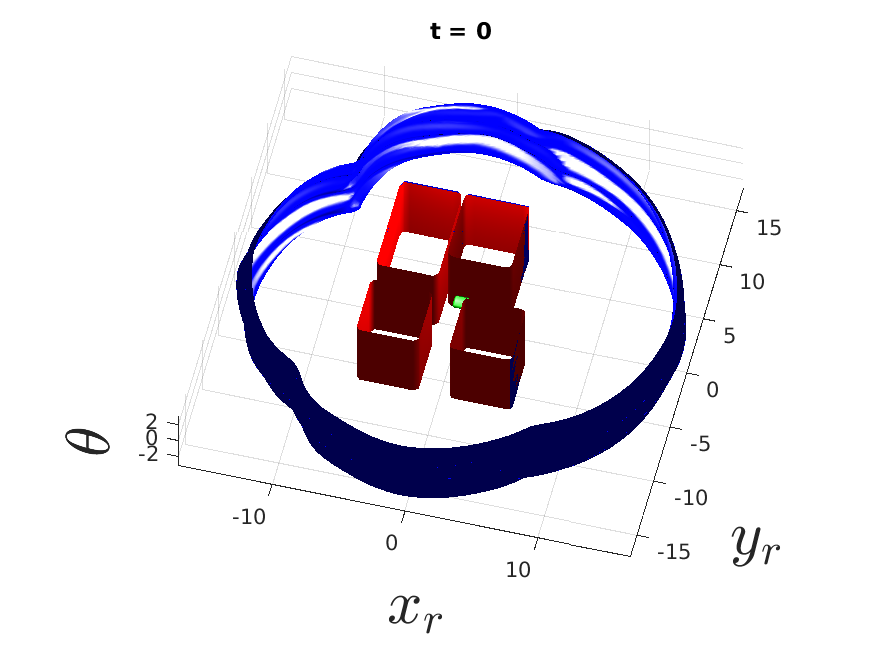
\includegraphics
        [width=0.4\textwidth]
        {figures/staticRAS3.png}
    \caption{The two horizontal axes represent the two first robot state components ($x_r$, $y_r$), while the third axis represents the third component $\theta$, namely the angle that the X-axis of $RF_m$ forms with $RF_w$. The small green cuboid represents the target set and four red cuboids representing the obstacles. Since this representation takes place in $\mathcal{C}$-space the obstacles are bigger than their real dimensions in the workspace and the target set seems smaller.}
    \label{fig:staticRAS3}
\end{figure}
\begin{figure}[h!]
    \centering
    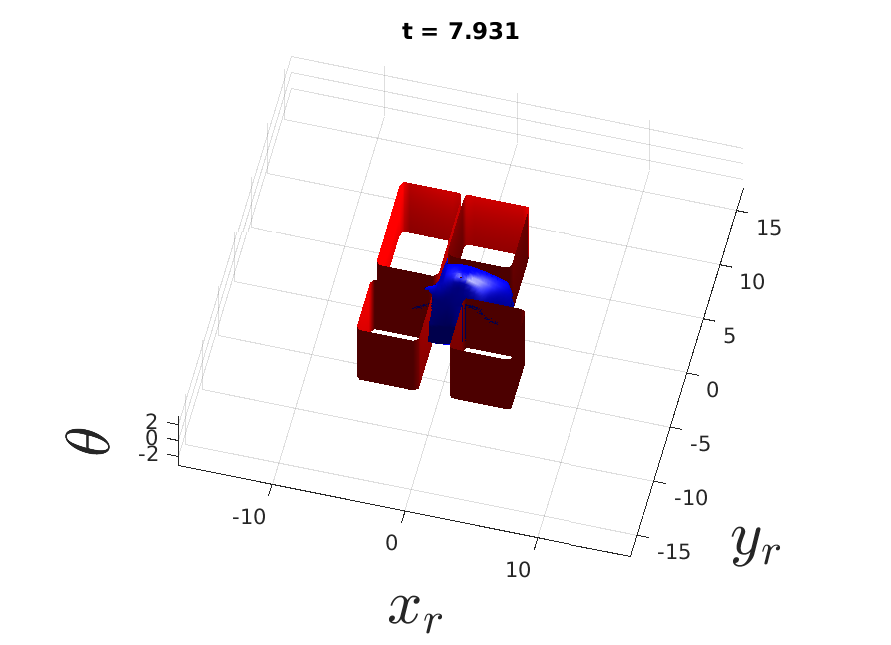
\includegraphics
        [width=0.4\textwidth]
        {figures/staticRAS2.png}
    \caption{Static environment and RAS at time 7.931s}
    \label{fig:staticRAS2}
\end{figure}
\begin{figure}[h!]
    \centering
    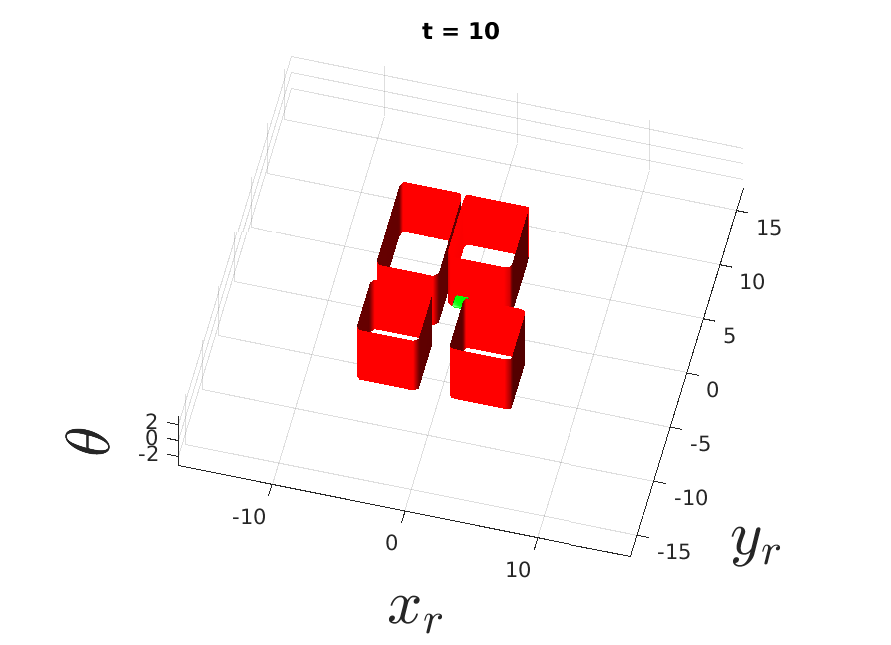
\includegraphics
        [width=0.4\textwidth]
        {figures/staticRAS1.png}
    \caption{Static environment and RAS at end game}
    \label{fig:staticRAS1}
\end{figure}
In $\mathcal{C}$-space the target set has a limited height $\theta \in [-0.1, 0.1]$ since we want the robot reaches the target set in the workspace with a desired orientation $\theta_d$ in a small range around $0\,rad$.

Now that the $RAS$ is defined we can see how the robot, starting from an initial state $x_0$ at time $t=0$, reaches the target set avoiding obstacles despite the disturbance. So since the robot's initial position $x_0 = [-5, -8 -2]$ is in the limits of the $RAS$ we can see that it reaches, after the needed time, the target set in the desired orientation, avoiding the obstacles in its path. Fig. (\ref{fig:static_opt}) shows the trajectory in both configuration and work-space and also the optimal player moves at each time instant of the game. In Fig. (\ref{fig:static_random}) is shown the same experiment but instead of an optimal disturbance we use a random one.
\begin{figure*}[hp!]
    \centering
    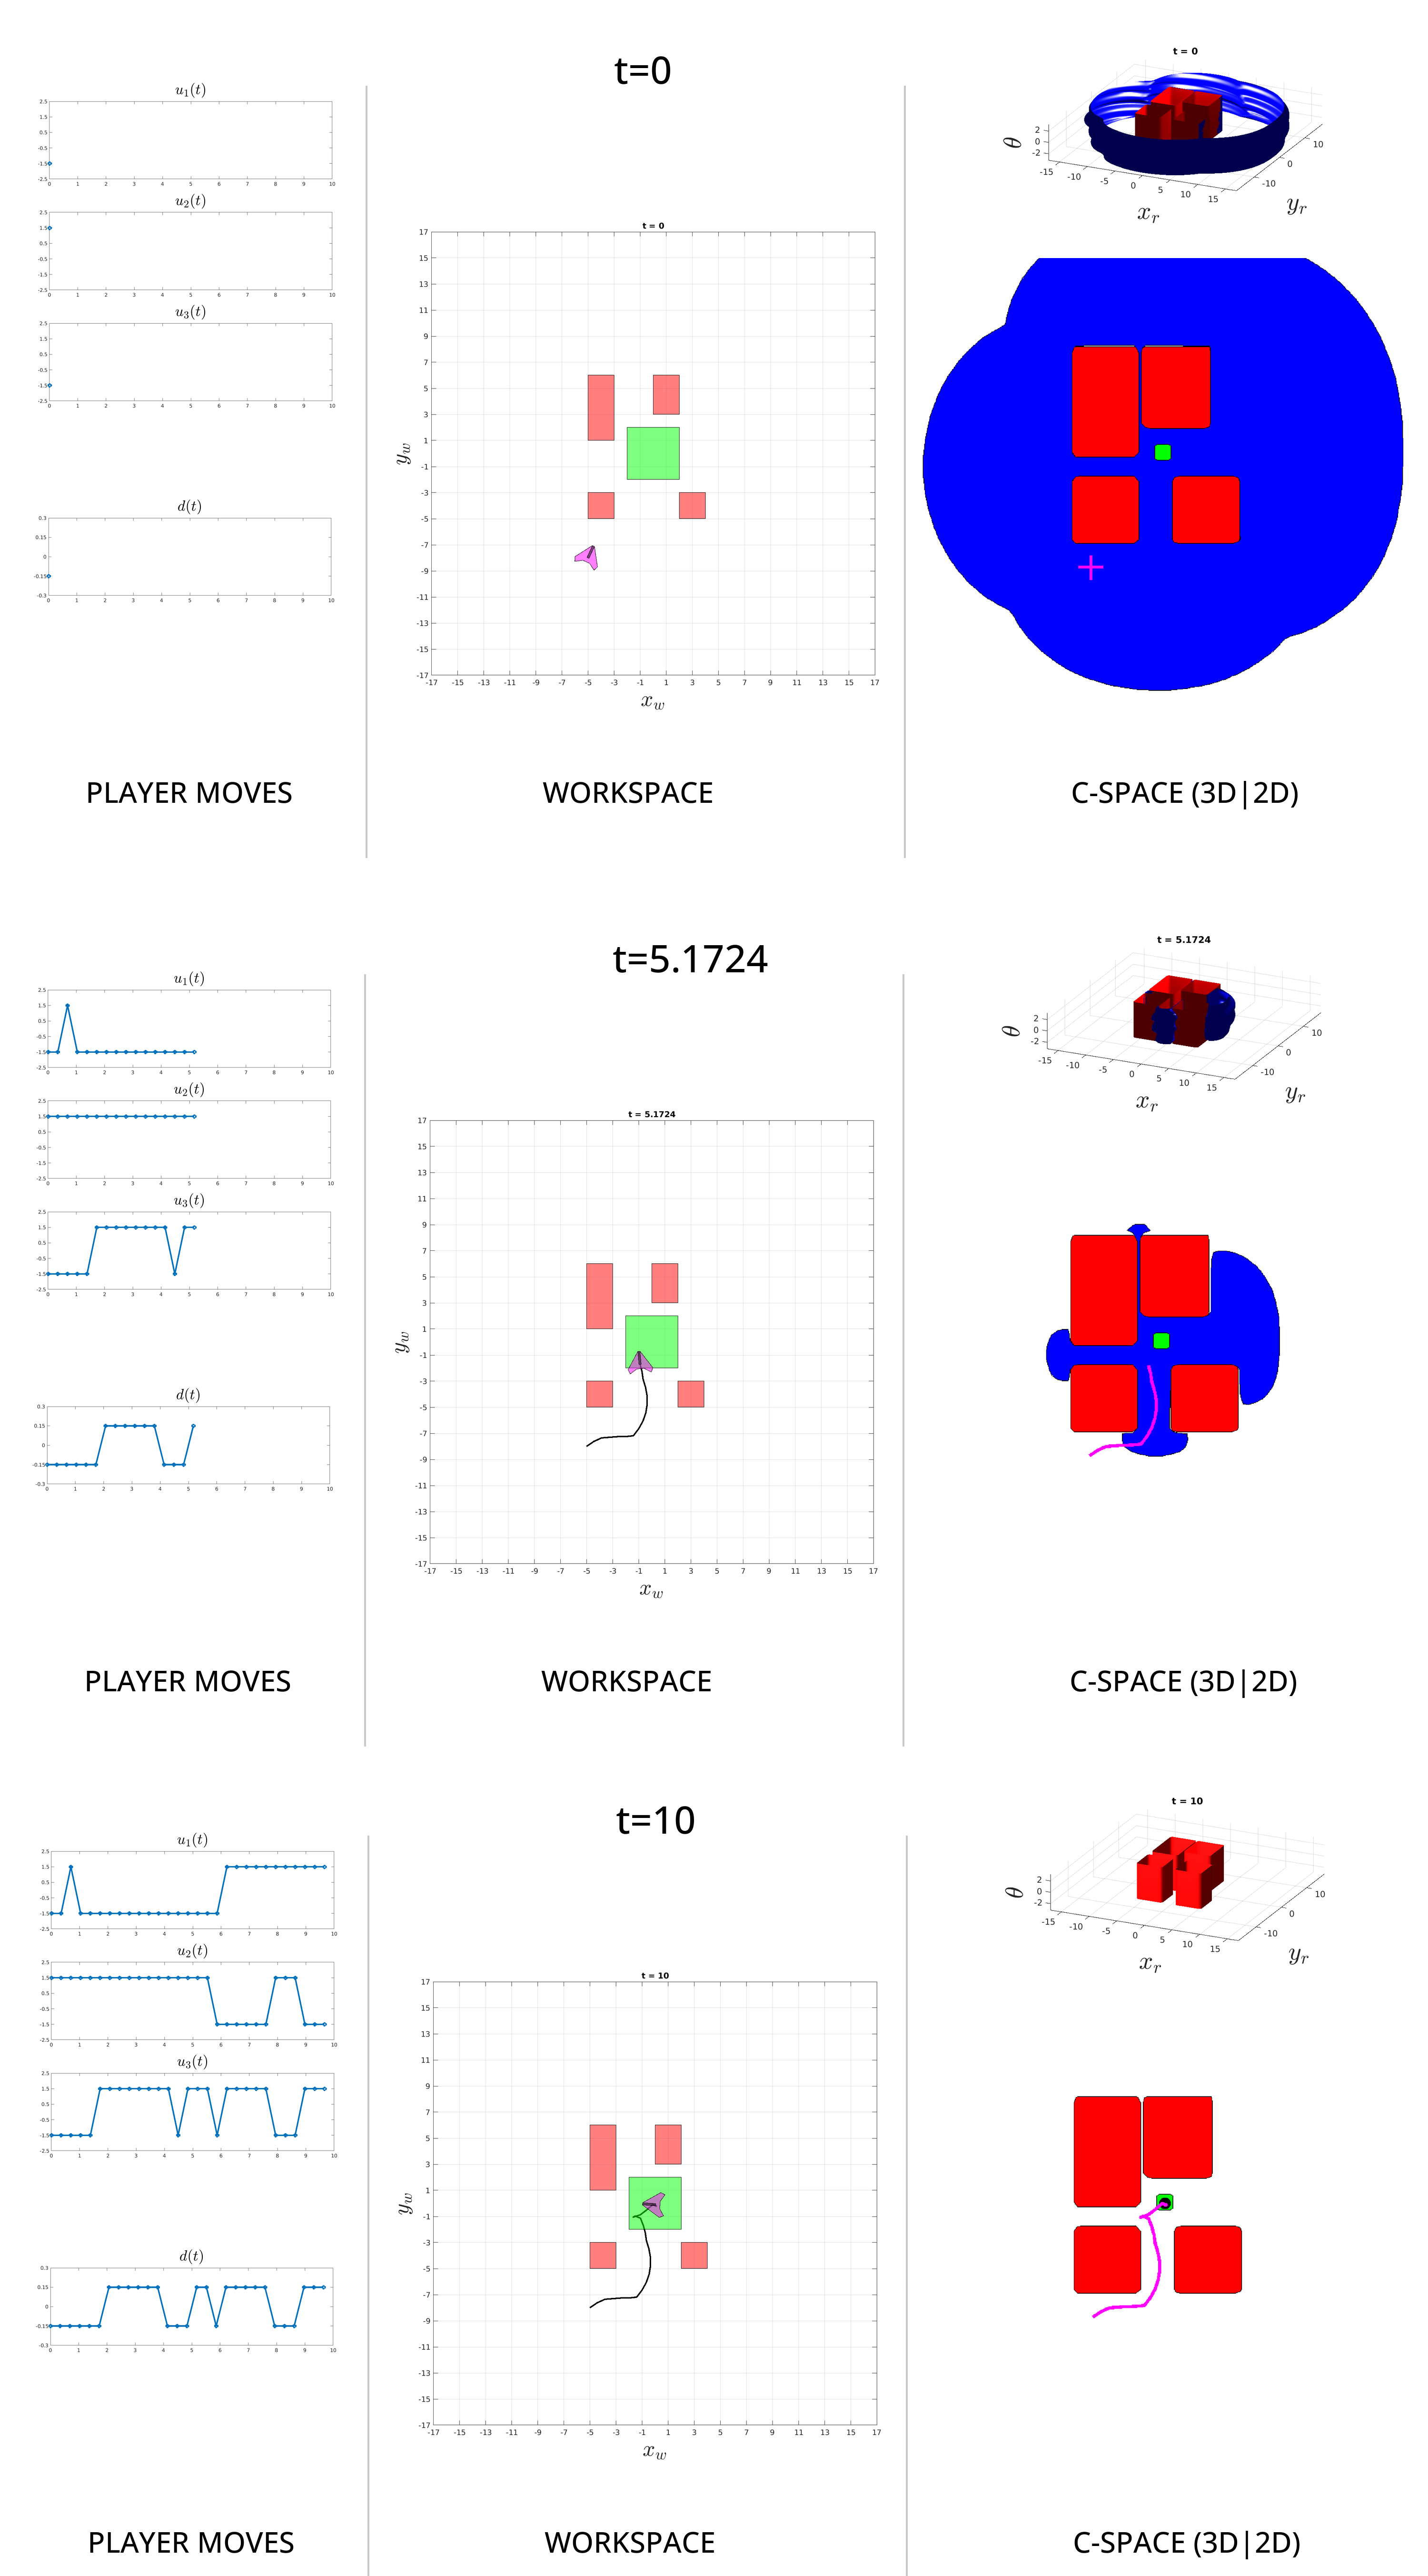
\includegraphics
        [width=0.7\textwidth]
        {figures/static_opt.png}
    \caption{Static environment, optimal disturbance. $x_0 = [-5, -8 -2]$, $\theta_d \in [-0.1, 0.1]$}
    \label{fig:static_opt}
\end{figure*}
\begin{figure*}[hp!]
    \centering
    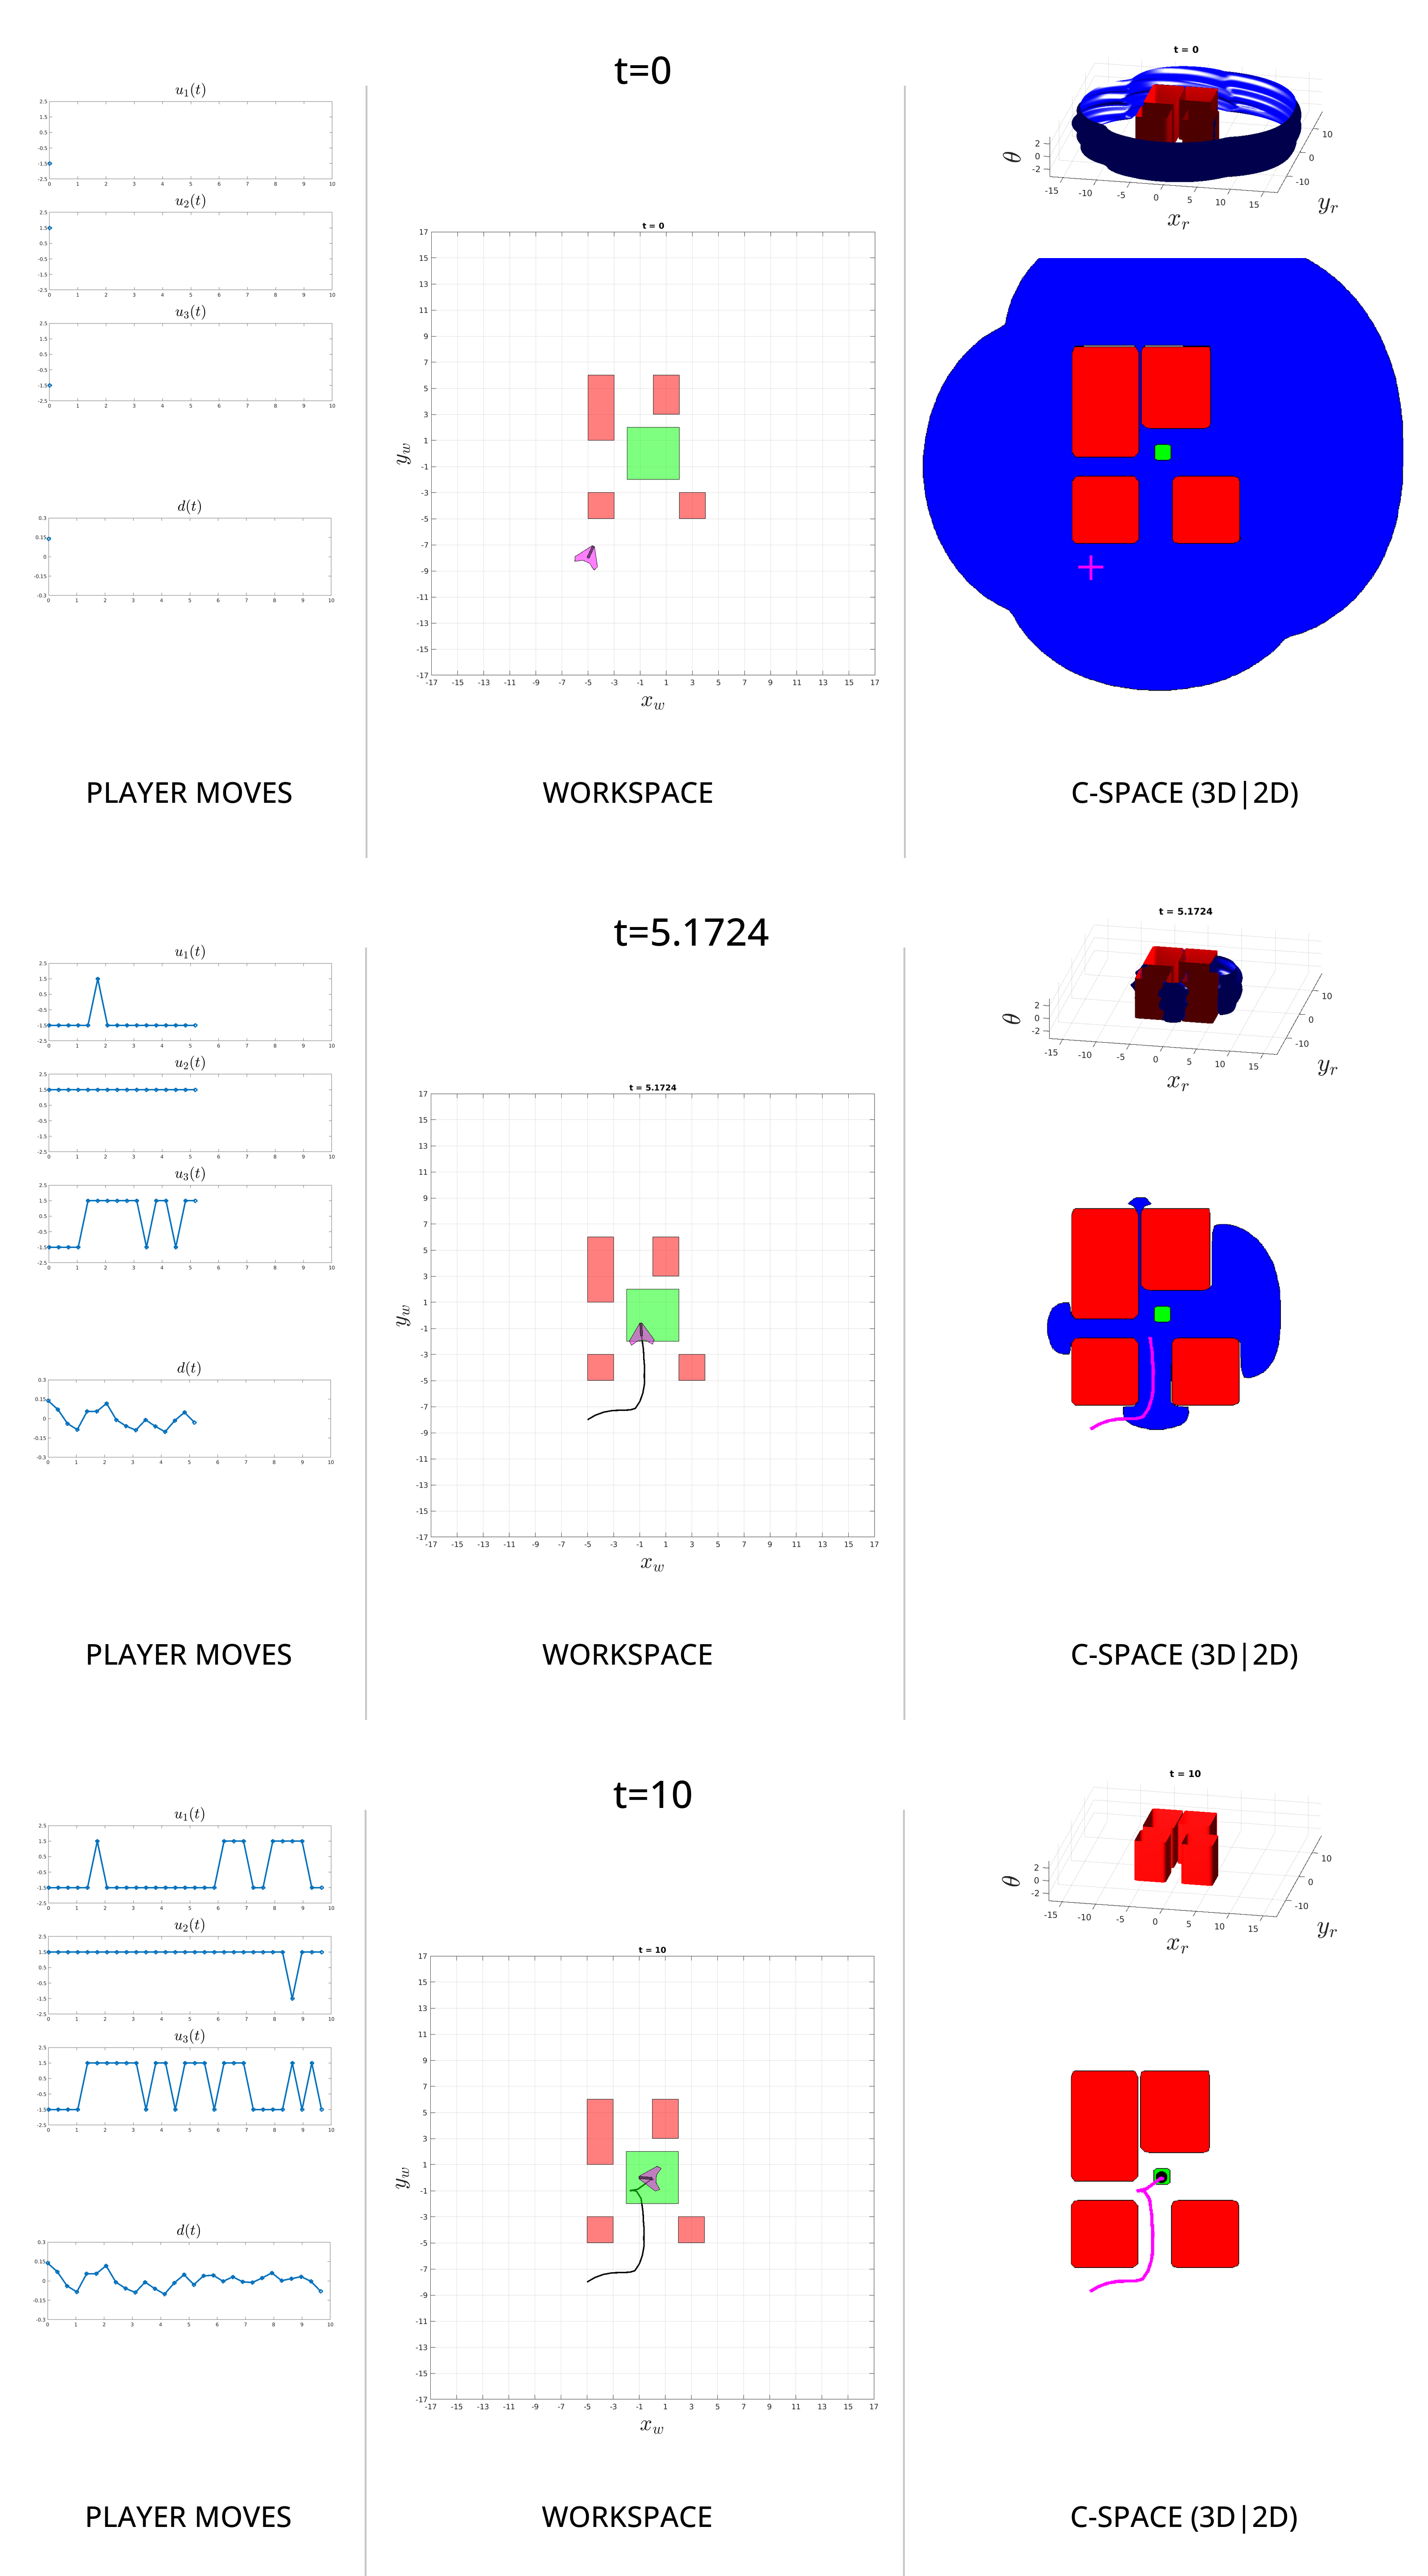
\includegraphics
        [width=0.7\textwidth]
        {figures/static_random.png}
    \caption{Static environment, random disturbance. $x_0 = [-5, -8 -2]$, $\theta_d \in [-0.1, 0.1]$}
    \label{fig:static_random}
\end{figure*}

%\pagebreak
\clearpage
%\newpage
\subsection{Dynamic Case}
Now we will see some more complex cases where reach set and avoid set are not fixed, but they move in the environment. Here we simulated a moving platform which represent a recharging station for the robot. So the robot has to access the platform while this platform is moving downward along the Y-axis. The platform is not accessible from everywhere, but only from the right side, while the other sides are surrounded by obstacles. 

As mentioned before, we simulated three different cases for the Dynamic experiments. 

We are going to see the $RAS$ developing over time in a particular direction since the target set (always represented by a green area) is moving. The next figure represents the $RAS$ at time 10 seconds (so still not expanded). As mentioned before this represents a platform that can be entered just by one side and surrounded by obstacles. Since we are always in the configuration space we can not see the small target set which is surrounded by the red obstacles which seem bigger in the C-space.
%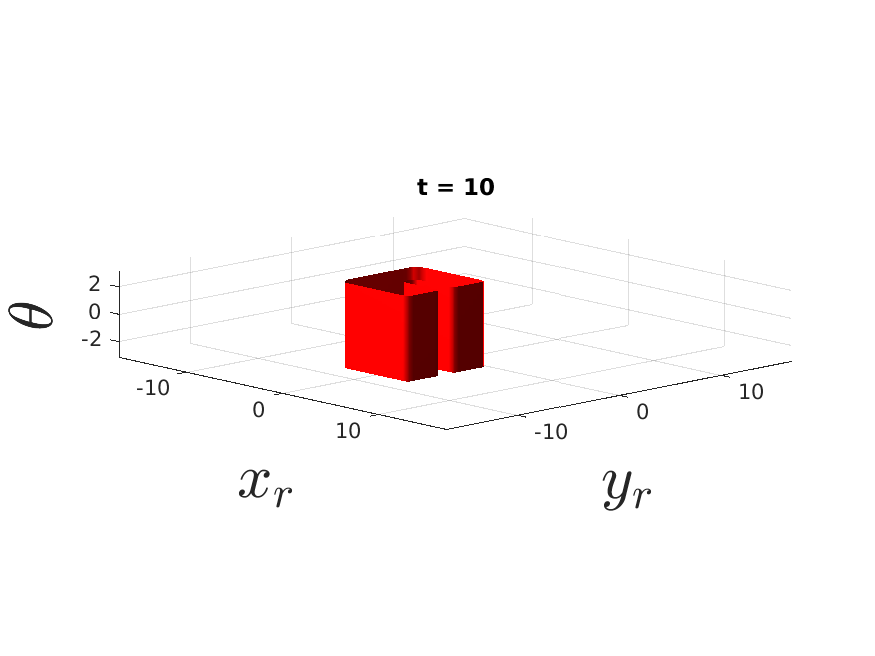
\includegraphics[scale=0.6]{dynamicRAS1.png}
At the end of the expansion of the $RAS$, so at time 0 seconds, we can see below the limits of the Set.
%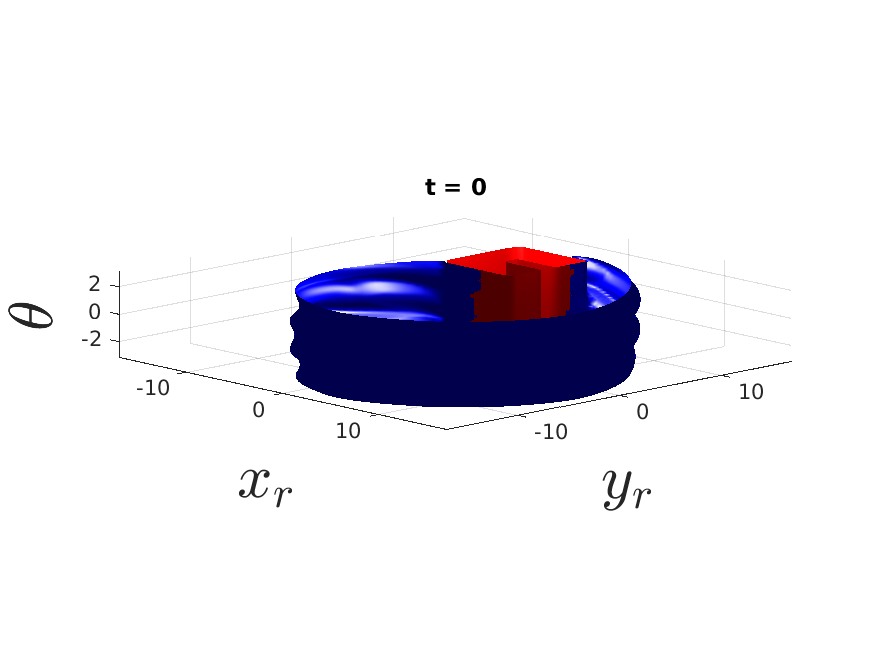
\includegraphics[scale=0.6]{dynamicRAS2.png}
We will see in each specific case a 2D representation of the $RAS$ to better understand the position of the target set and the different initial positions of the robot.
\subsubsection{Case 1}
In this first case the initial position of the robot is relatively near the target set and inside the $RAS$ at time 0 seconds, so we know from the theory that exists a trajectory which can lead the robot inside the target set in the maximum given time (10 seconds).
%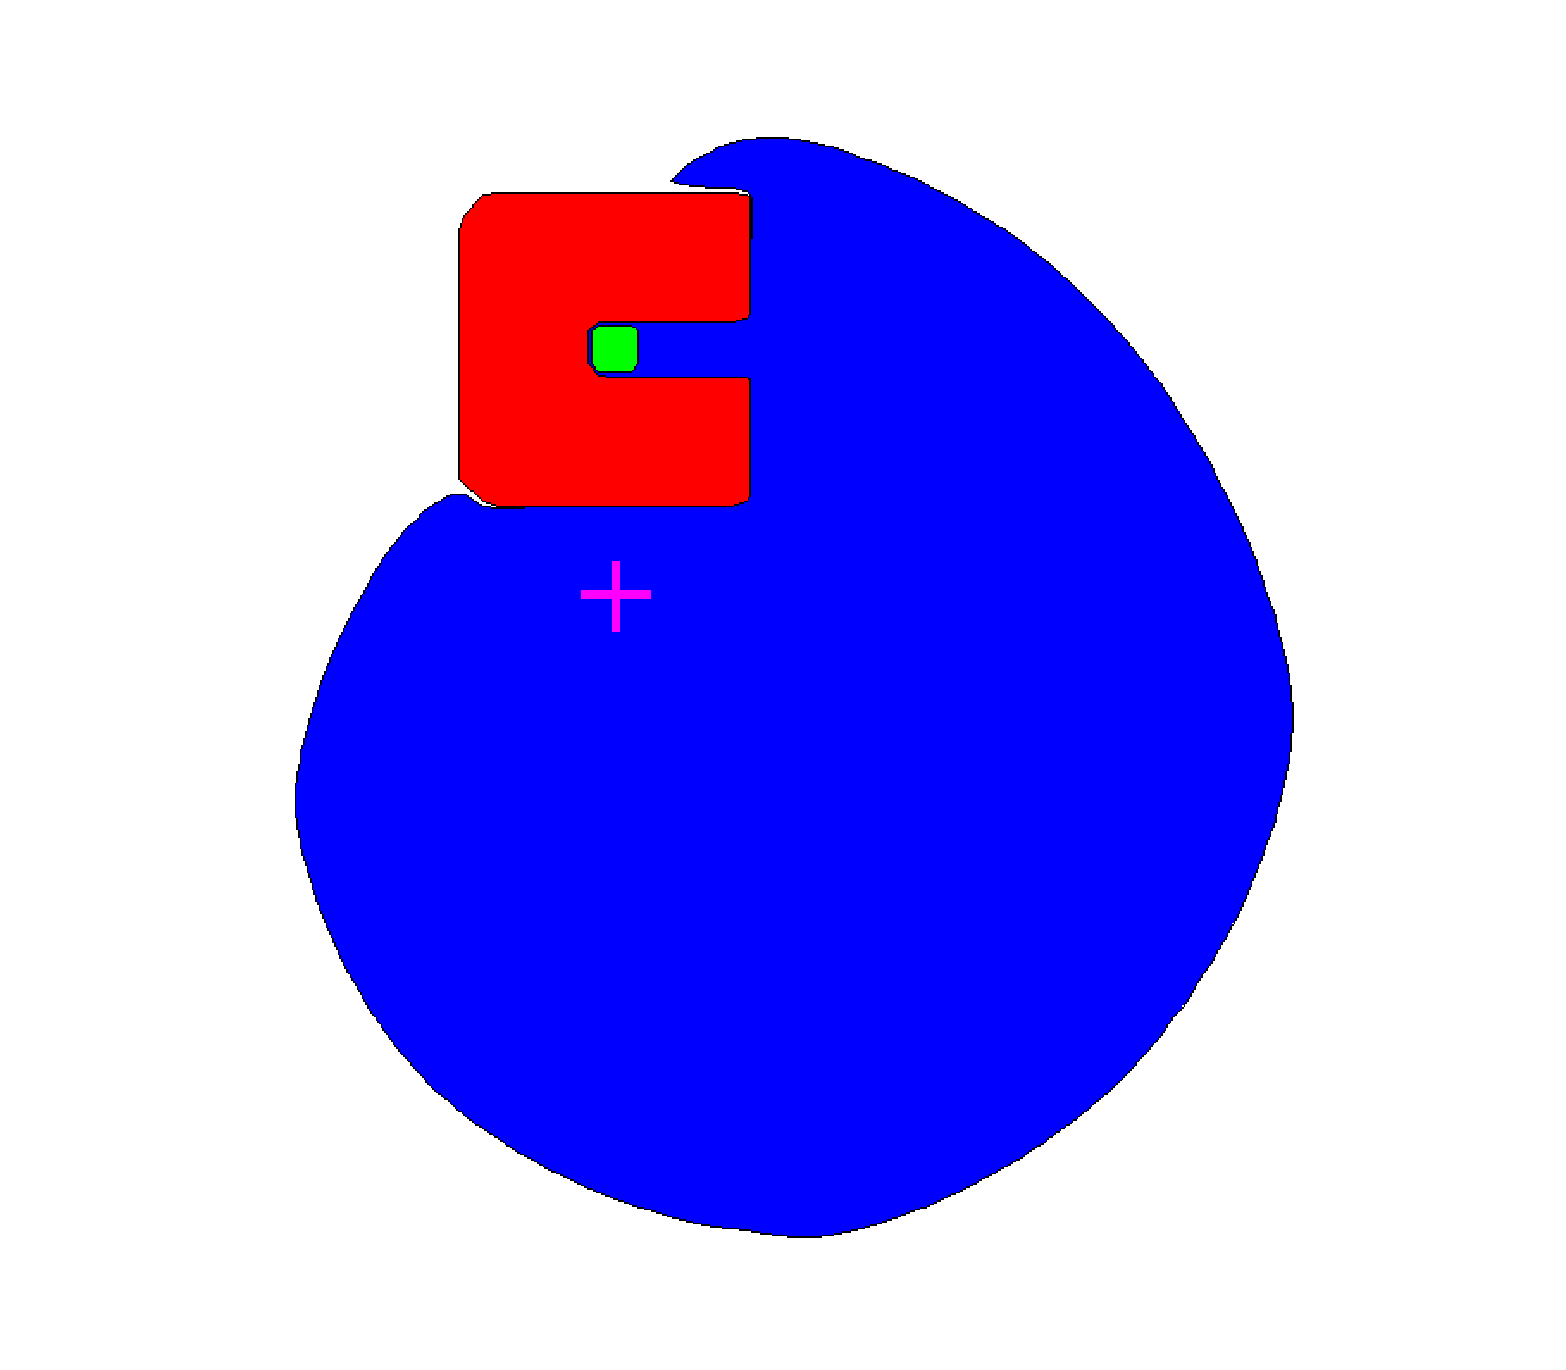
\includegraphics[scale=0.25]{dynamic2Dras1.png}
%\\
In the figure we have the 2D $RAS$ (The blue area), The obstacles (Red Area), The target set (The green area) and the initial configuration of the robot (The pink cross). From this plot we can not see the initial angular orientation of the robot since is a 2D representation, but we can better understand it from the trajectory plots below. It is important to say that the target set is not restricted only in small area of the X-axis and Y-axis , but is also limited in terms of the desired target angel $\theta$ (like in the static case). In this case we set as desired $\theta$ a small range around the angle 0 $rad$. The initial position of the robot is $x=0$ and $y=0$.
%\\
%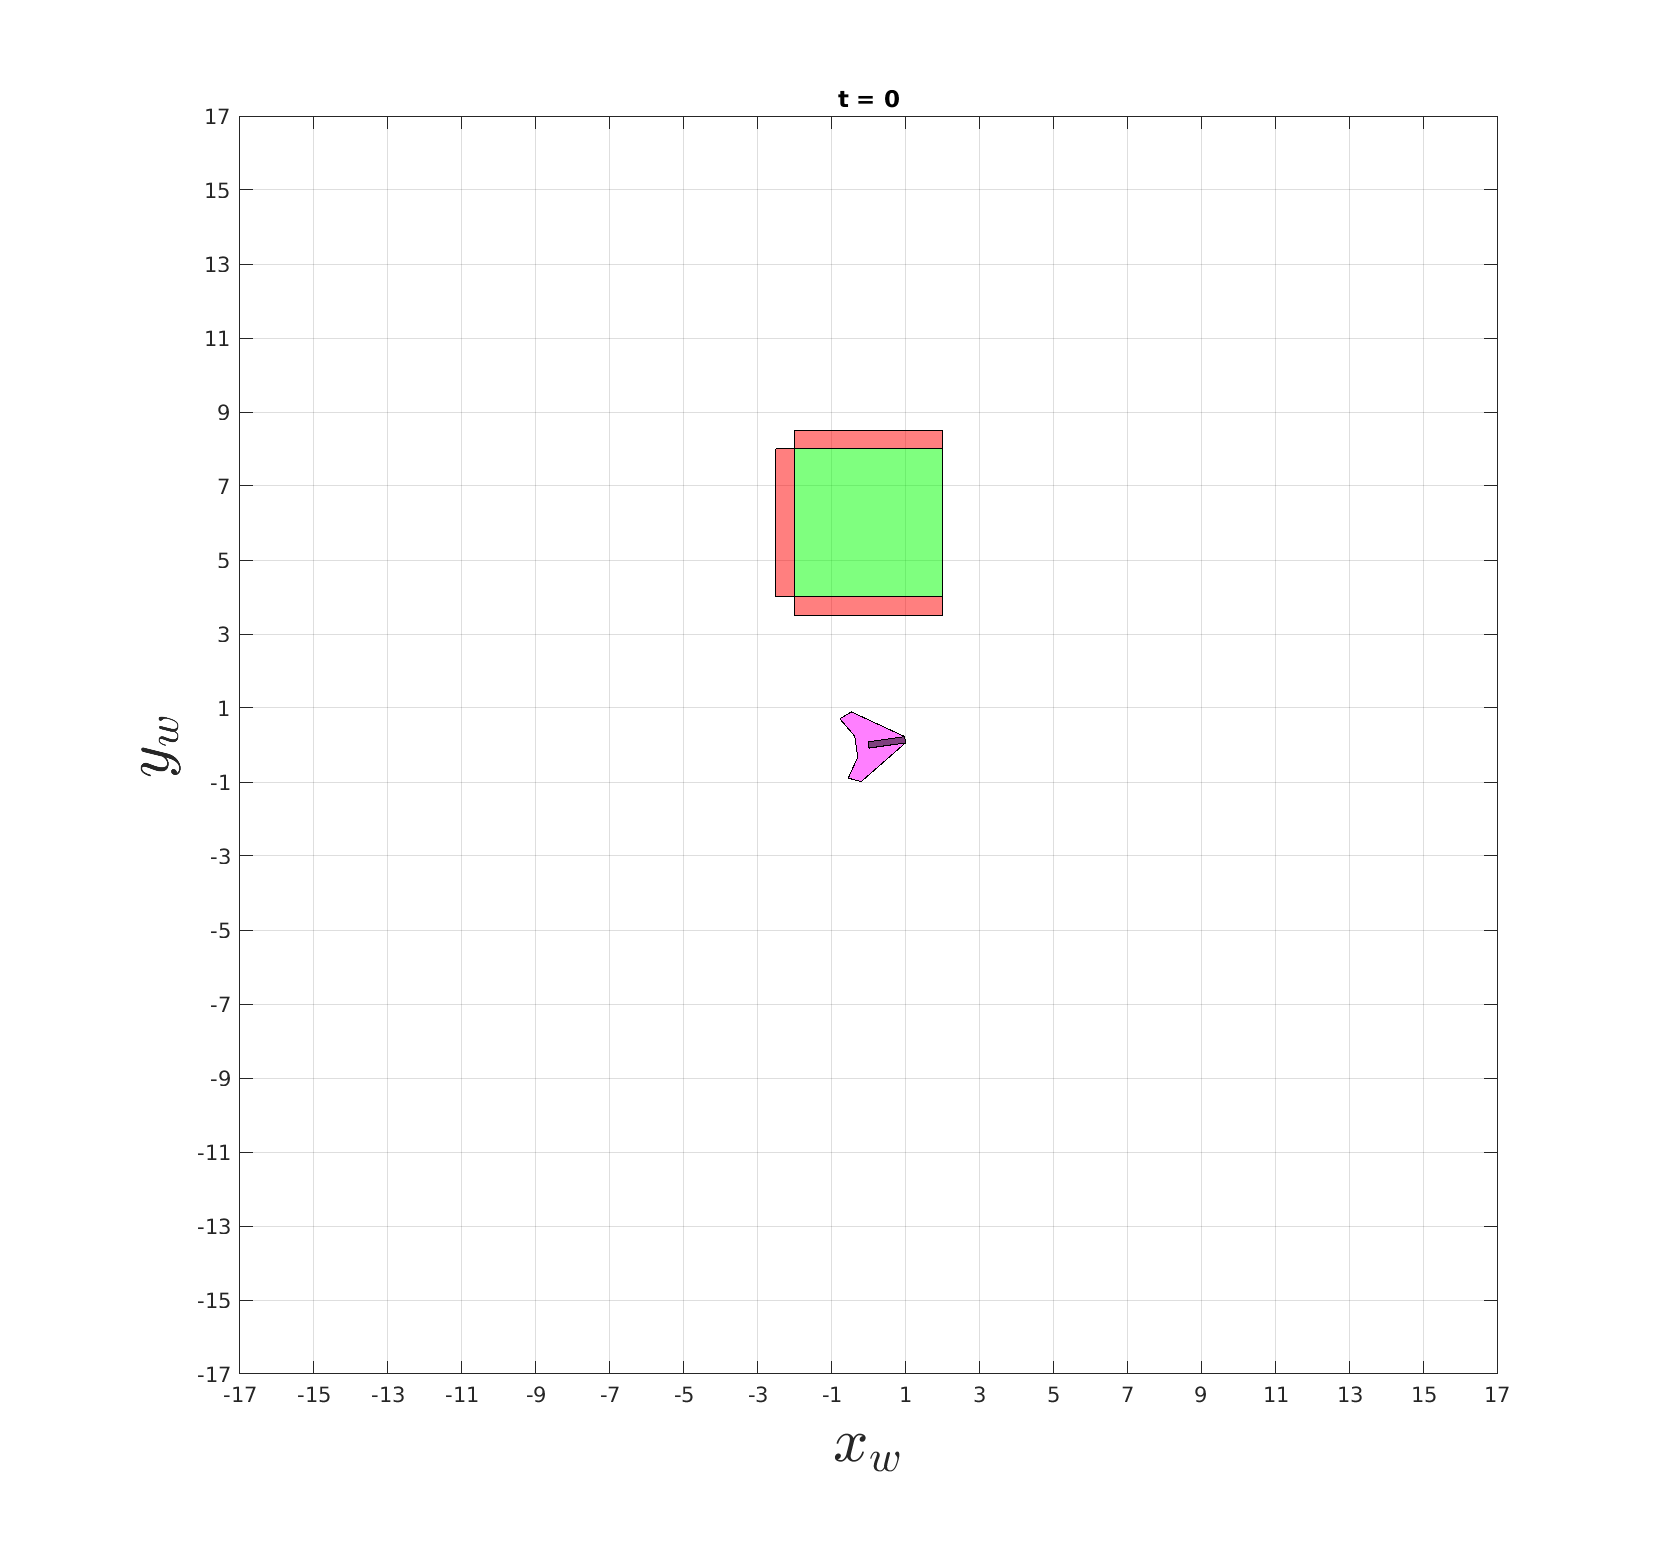
\includegraphics[scale=0.25]{dynamicTRAJ1.png}
%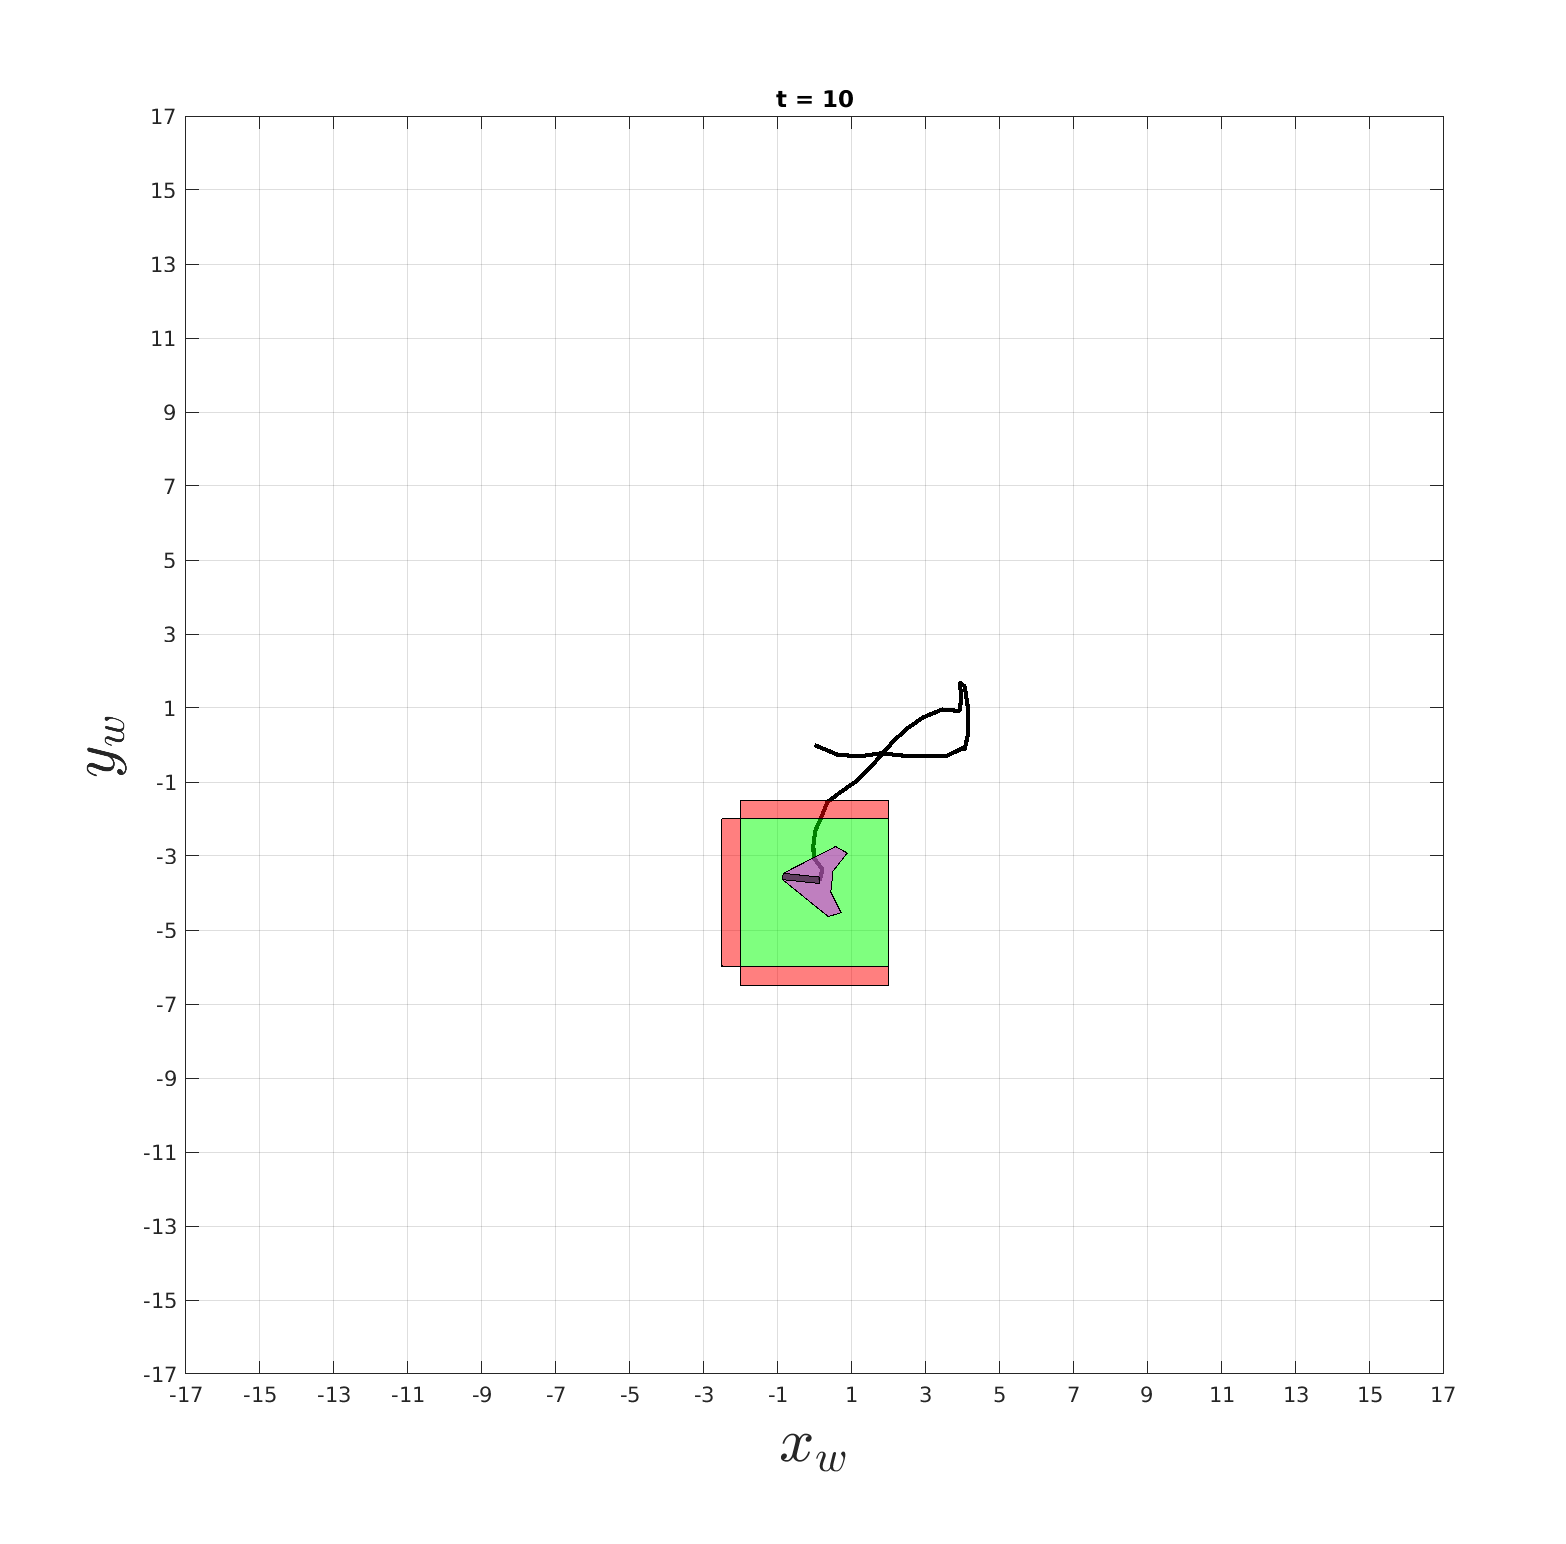
\includegraphics[scale=0.25]{dynamicTRAJ2.png}
%\\
We can see here the particular trajectory of the robot due to the movement of the target set. At time $t=10sec$ the robot is in the target set without collisions with the obstacles as expected. We can also see how it enters the target set with the desired angulation around the radiant 0

\subsubsection{Case 2}
The second case is similar to the previous one. In this case the only difference with the first one is the initial position of the robot. Here the robot is relatively distant from the target set, but still in the $RAS$. 
%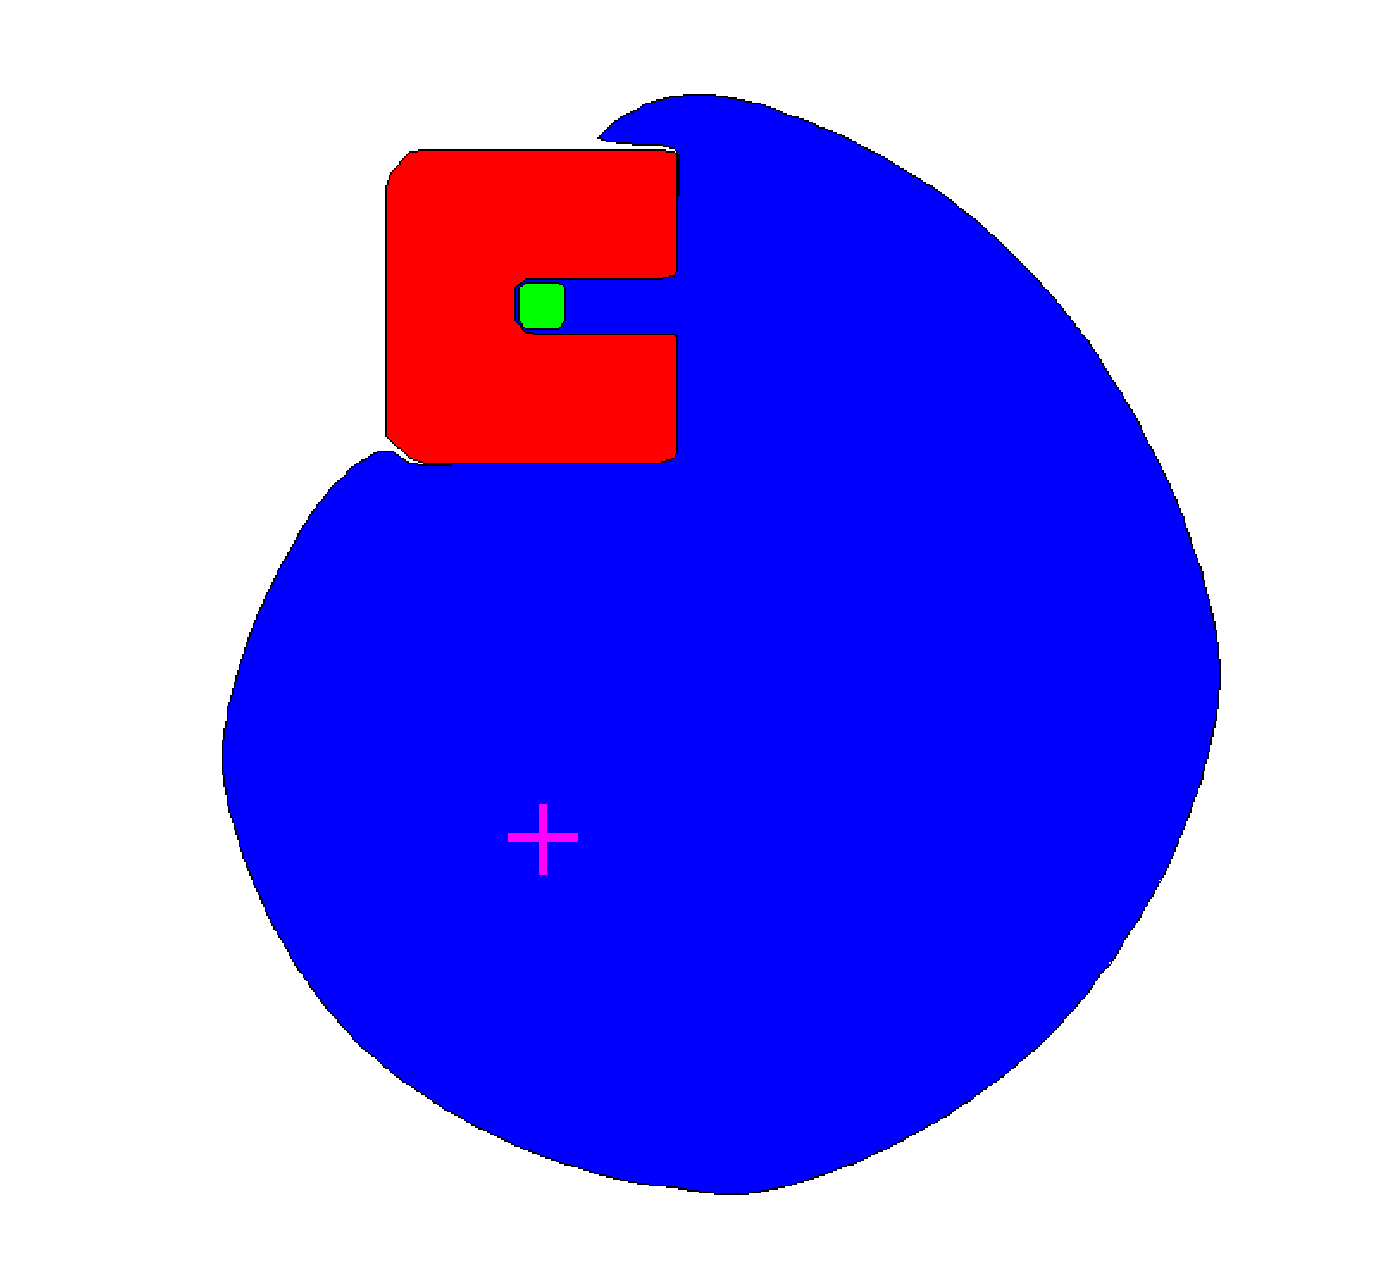
\includegraphics[scale=0.25]{dynamic2Dras2.png}
%\\
Since its initial position is still in the limits of the $RAS$ we can compute the following trajectory with robot's initial position $x=0$ and $y=-7$.
%\\
%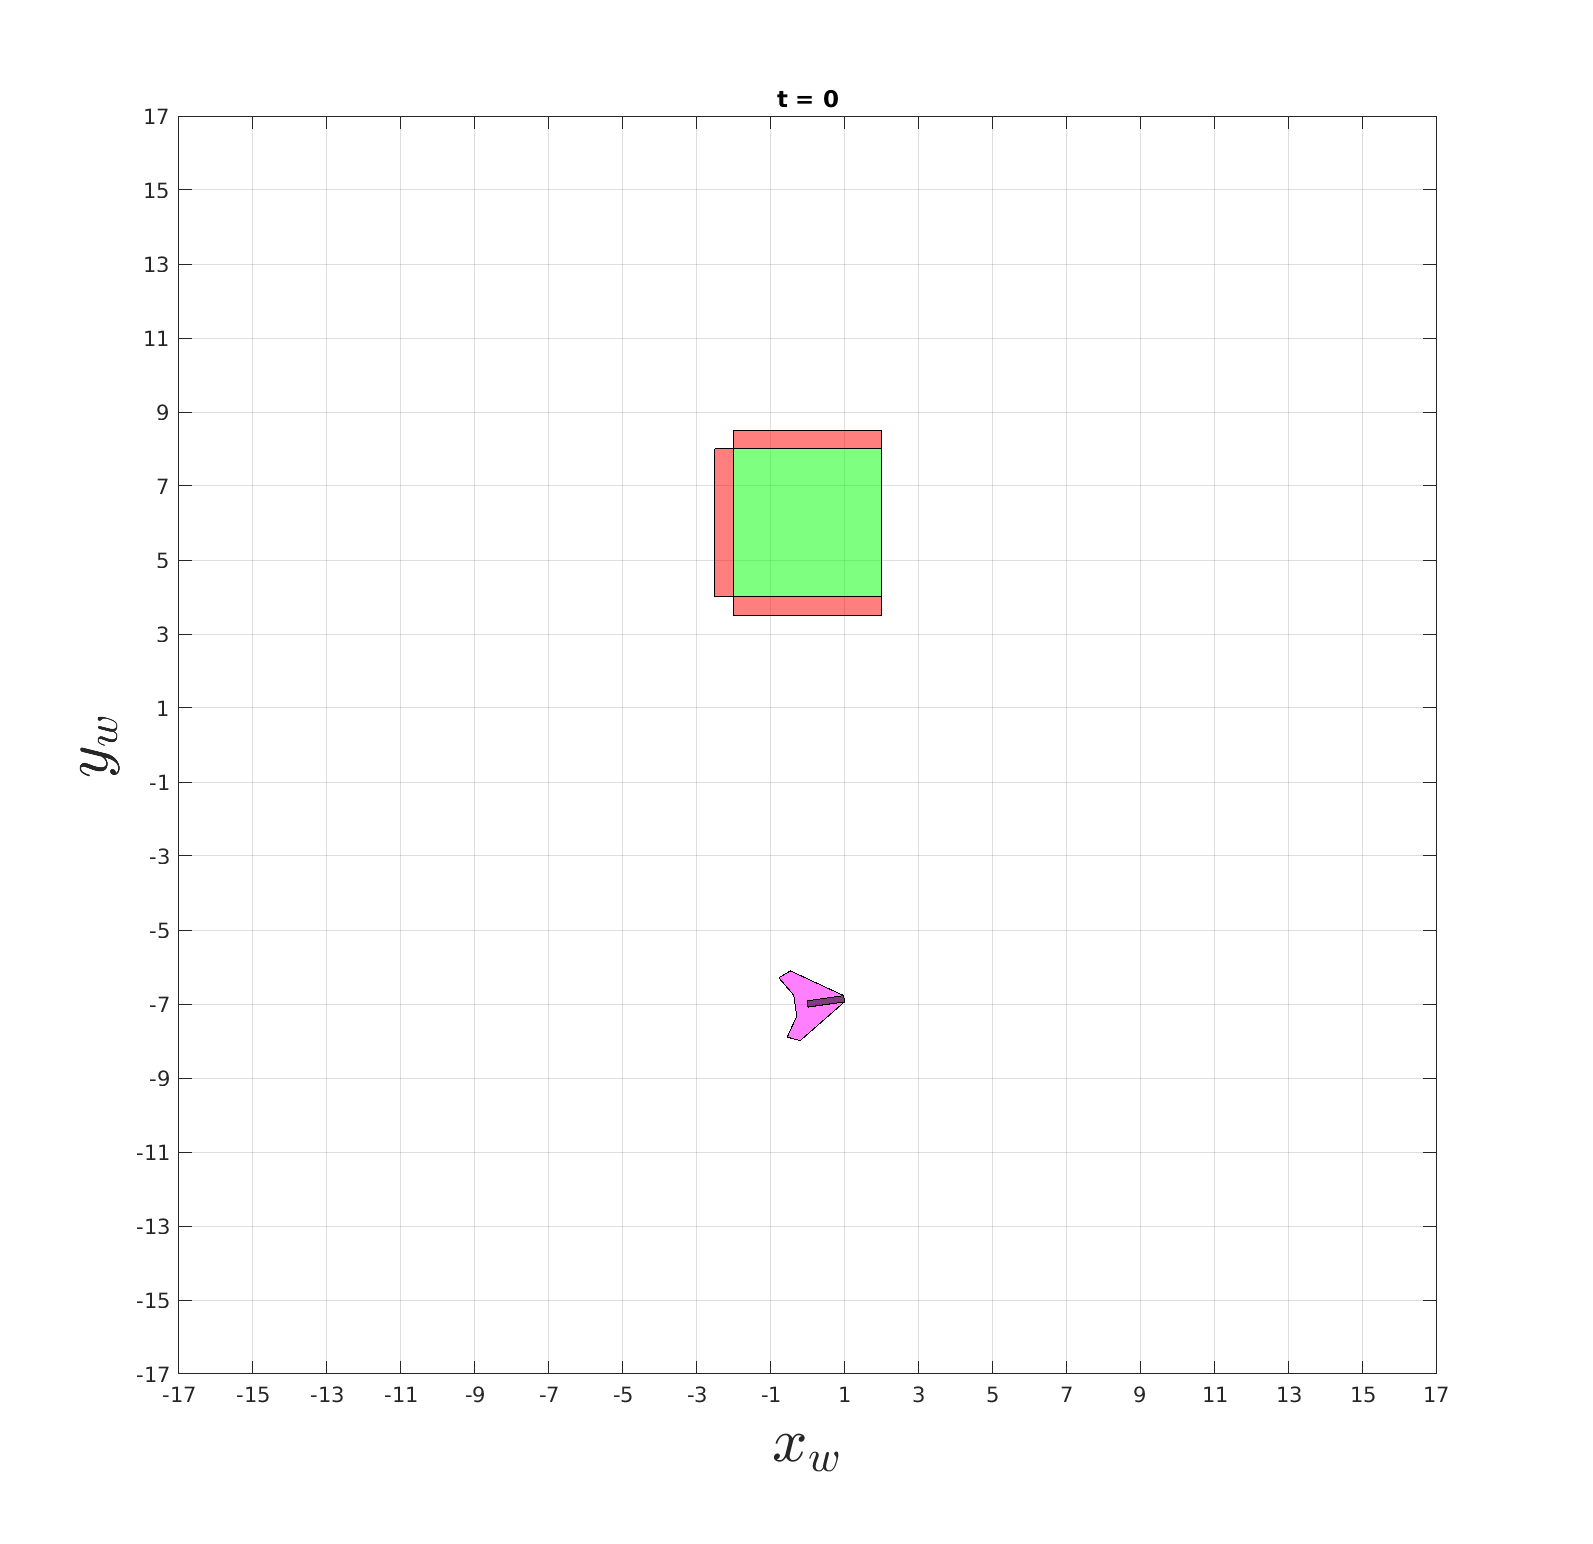
\includegraphics[scale=0.25]{dynamicTRAJ3.png}
%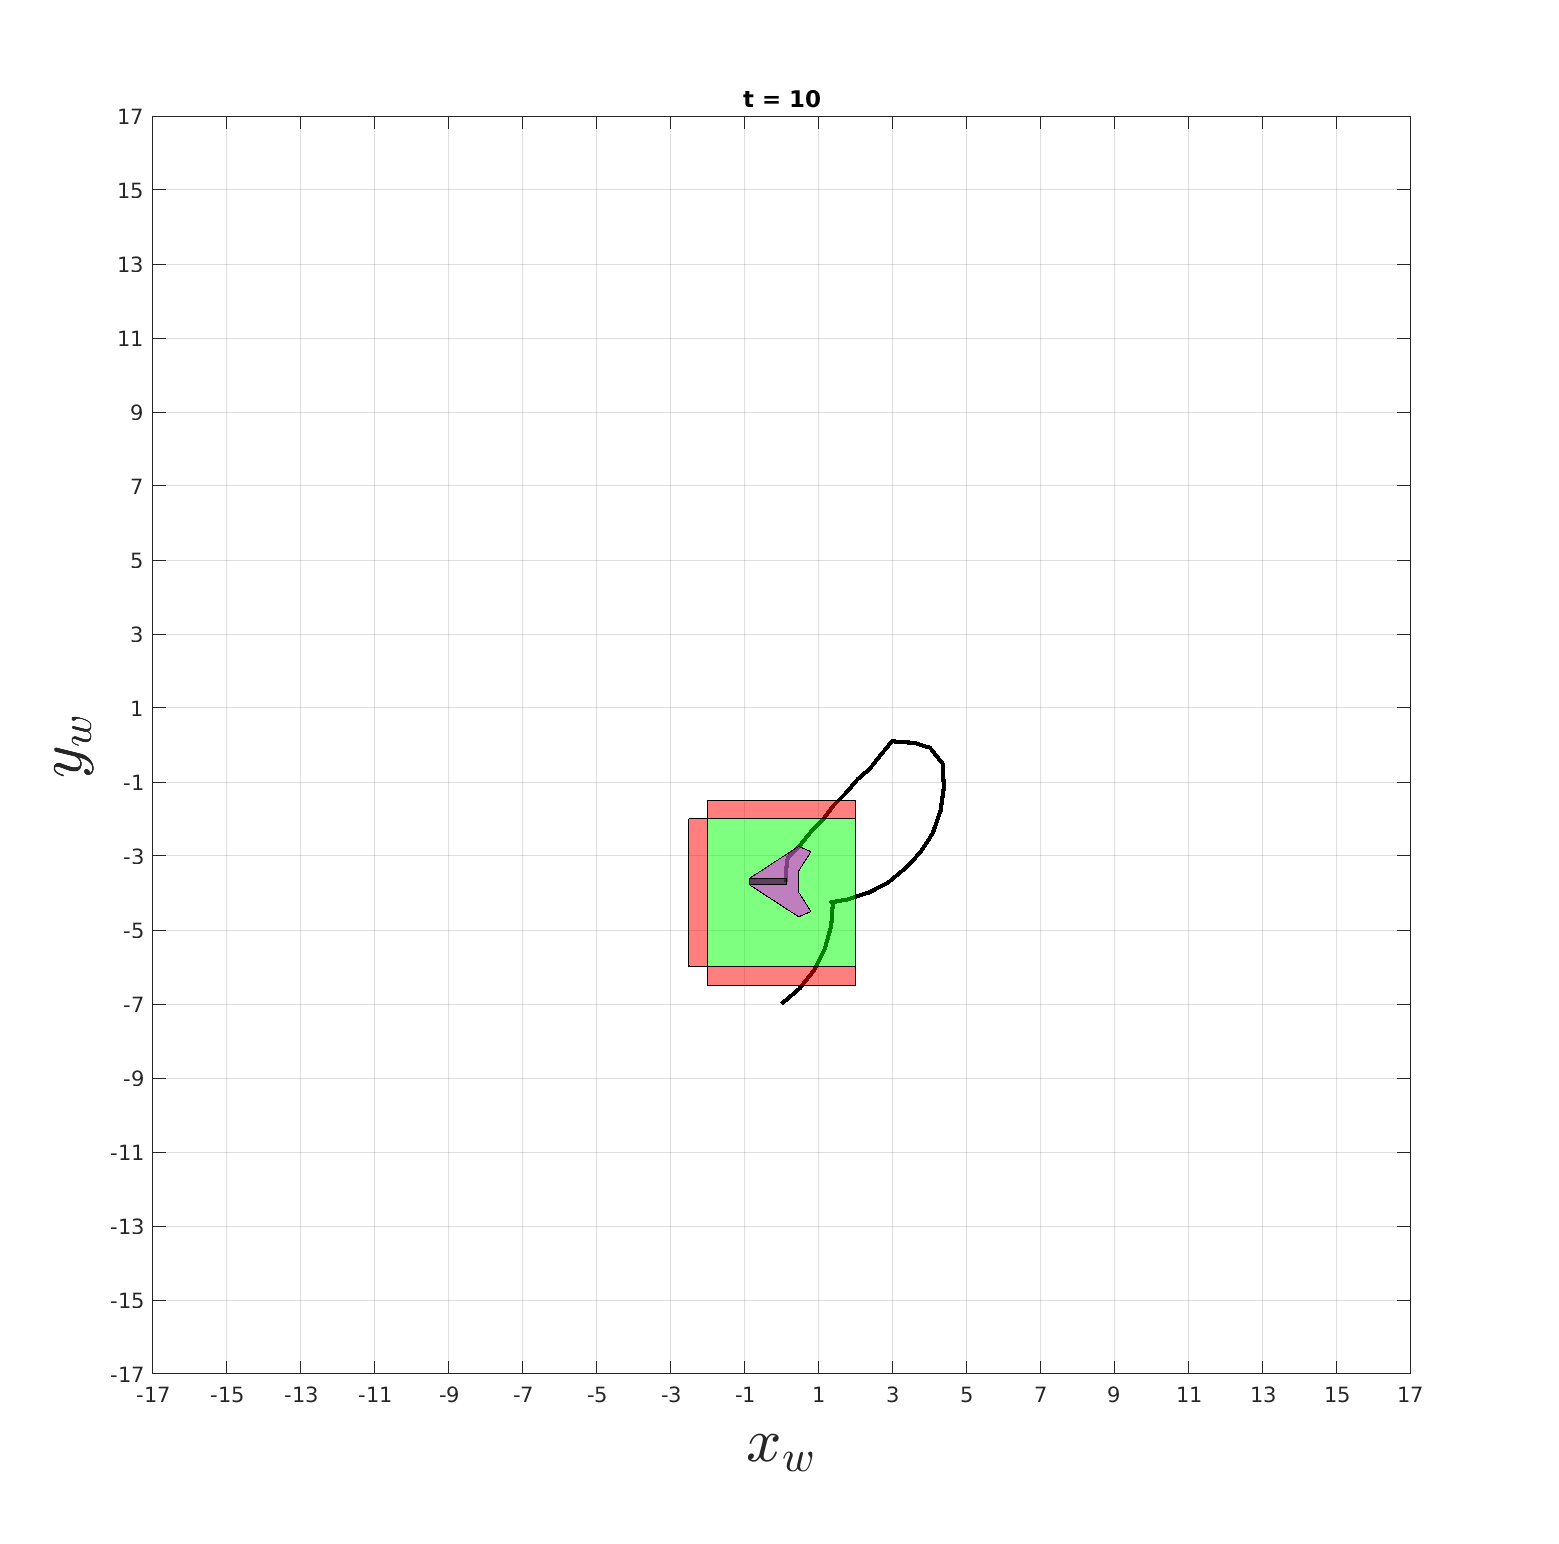
\includegraphics[scale=0.25]{dynamicTRAJ4.png}
%\\
Even in this case the Robot successfully reached the target set with the desired target angle $\theta=0$, playing against the optimal disturbance and avoiding any obstacle.

\subsubsection{Case 3}
In this last case we see what happens if the initial position of the robot is outside the $RAS$. 
%\\
%\includegraphics[scale=0.20]{dynamic2Dras3.png}
%\\
The initial position of the robot is $x=14$ and $y=14$, so completely outside the bounds of the Reach-Avoid Set.
Obviously we can already say that the robot is not going to reach the Target Set.
%\\
%\includegraphics[scale=0.25]{dynamicTRAJ5.png}
%\includegraphics[scale=0.25]{dynamicTRAJ6.png}
%\\
At time $t=10 seconds$ the robot is still outside the target set since the expansion of the $RAS$ was not big enough to include the robot at its initial position.
        

\begin{figure*}[hp!]
    \centering
    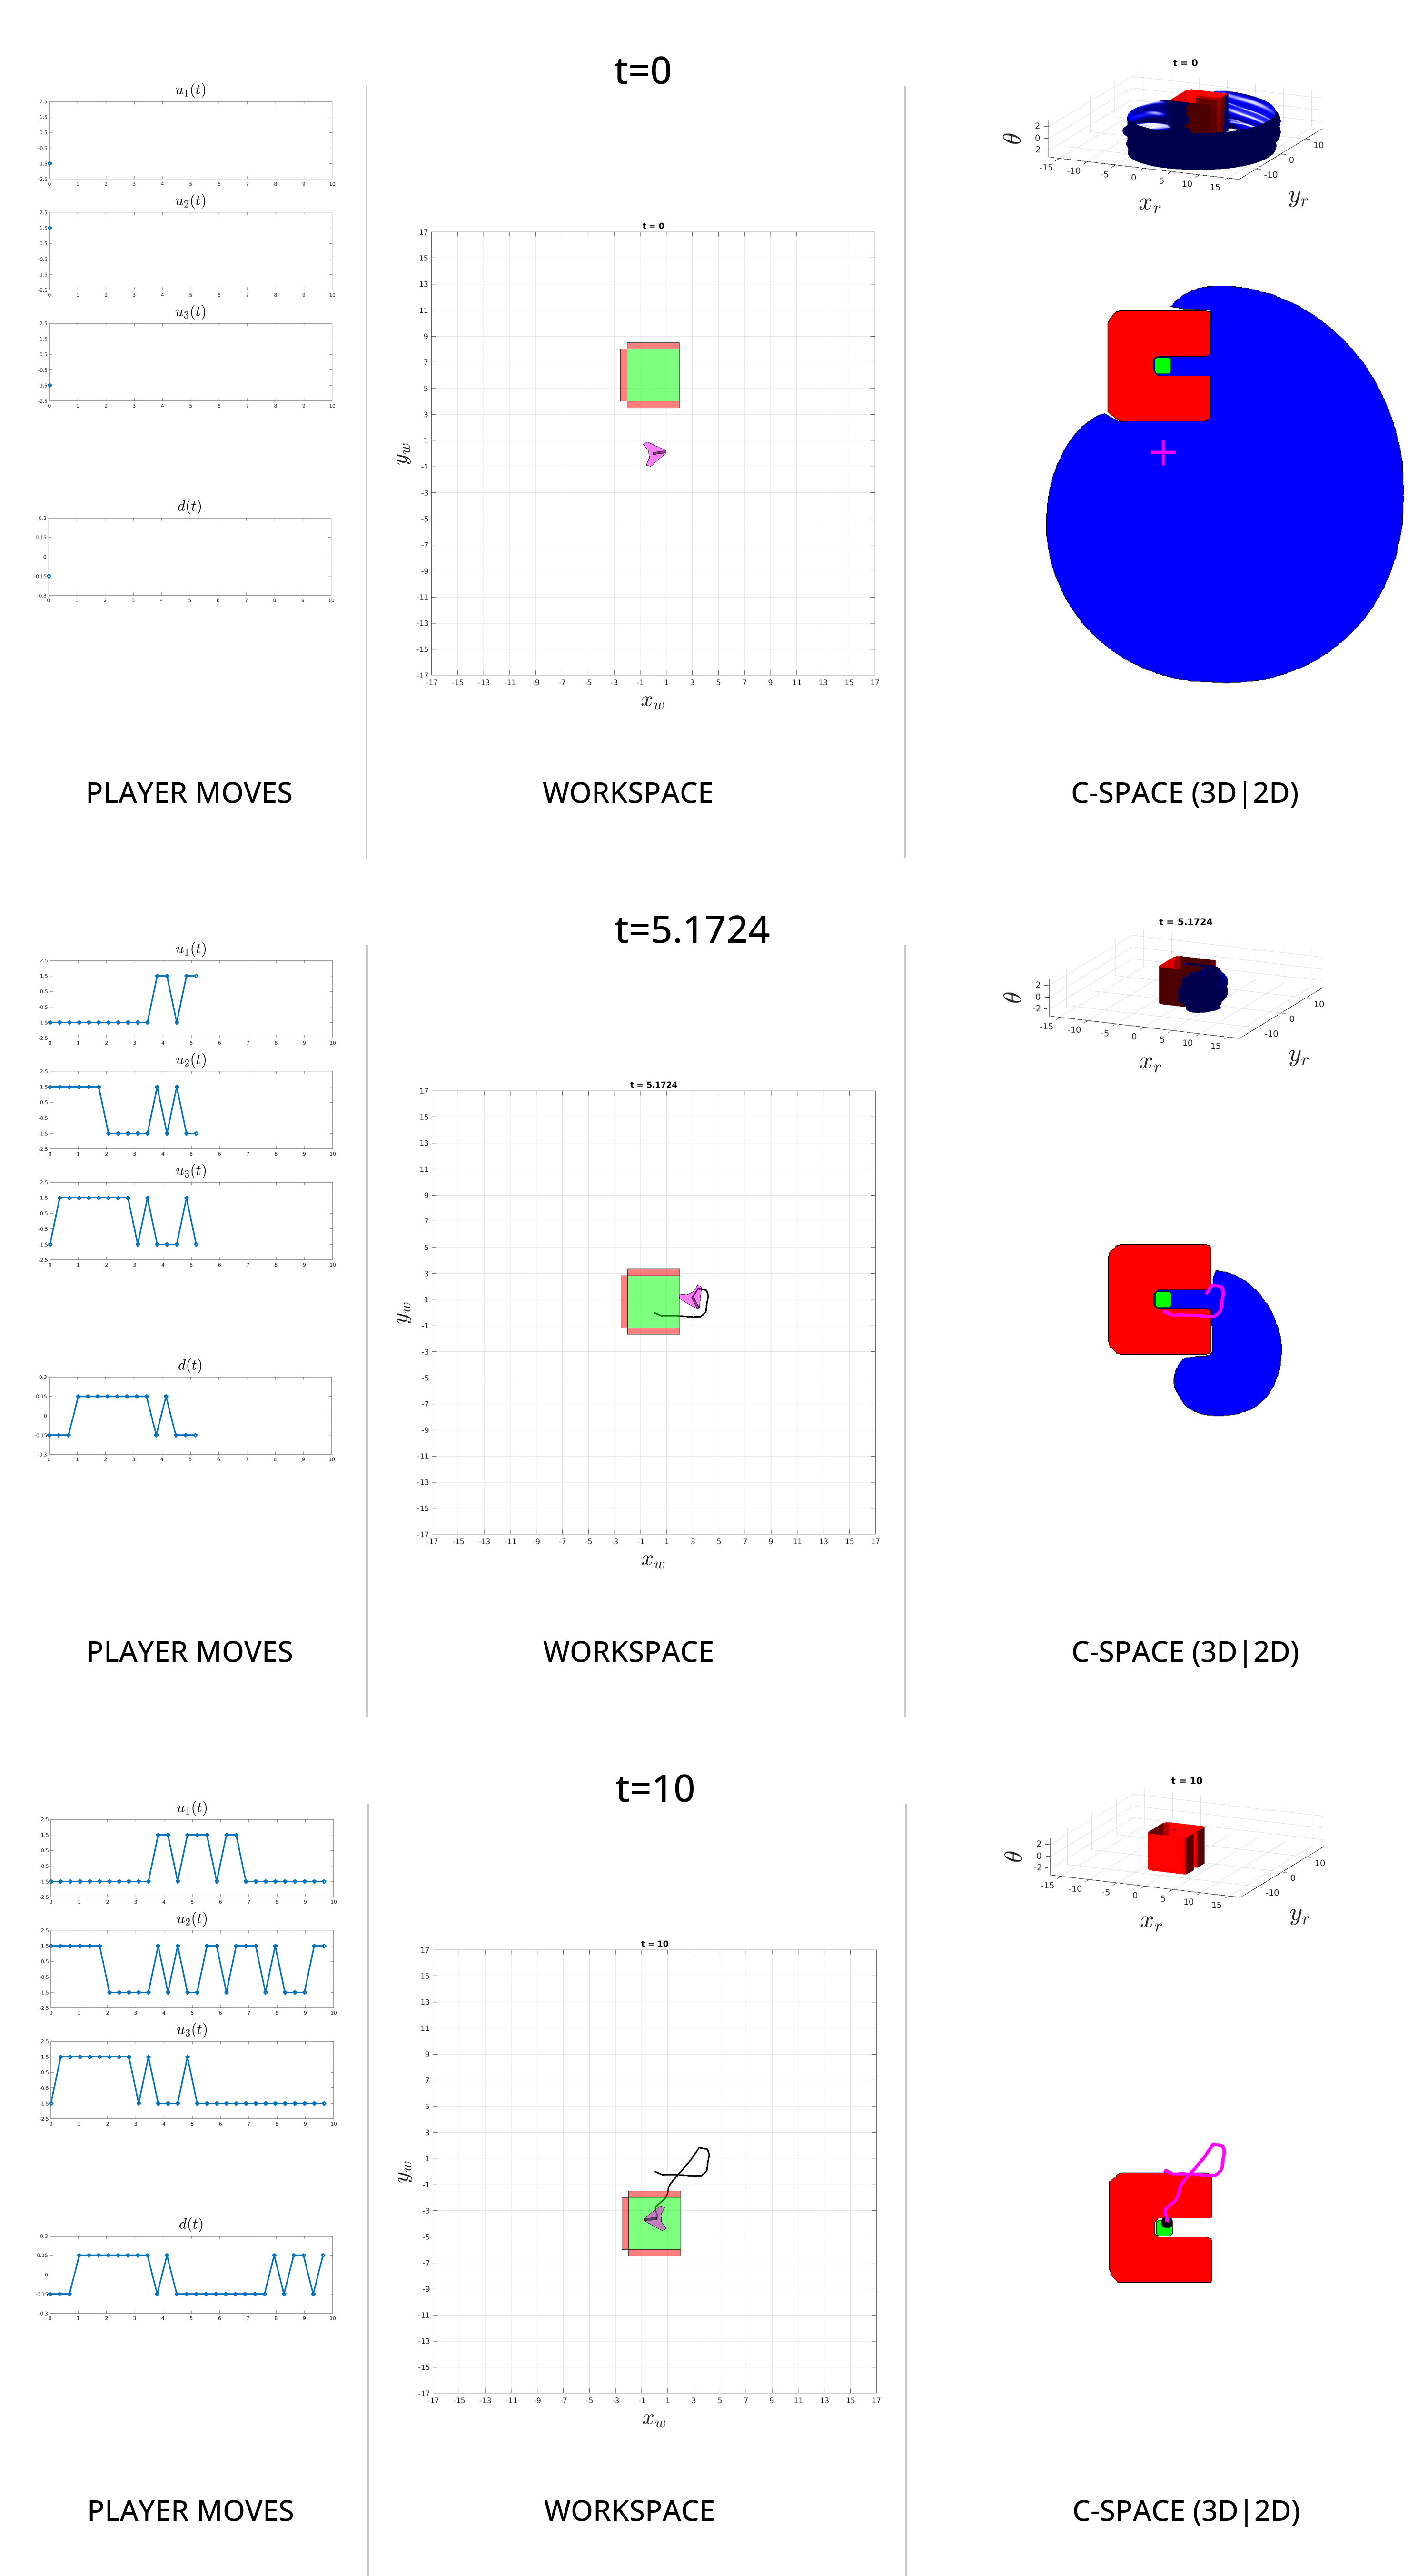
\includegraphics
        [width=0.7\textwidth]
        {figures/dynamic_closer_opt.png}
    \caption{Dynamic environment, optimal disturbance. $x_0 = [0, 0, -3]$, $\theta_d \in [-0.1, 0.1]$}
    \label{fig:dynamic_closer_opt}
\end{figure*}

\begin{figure*}[hp!]
    \centering
    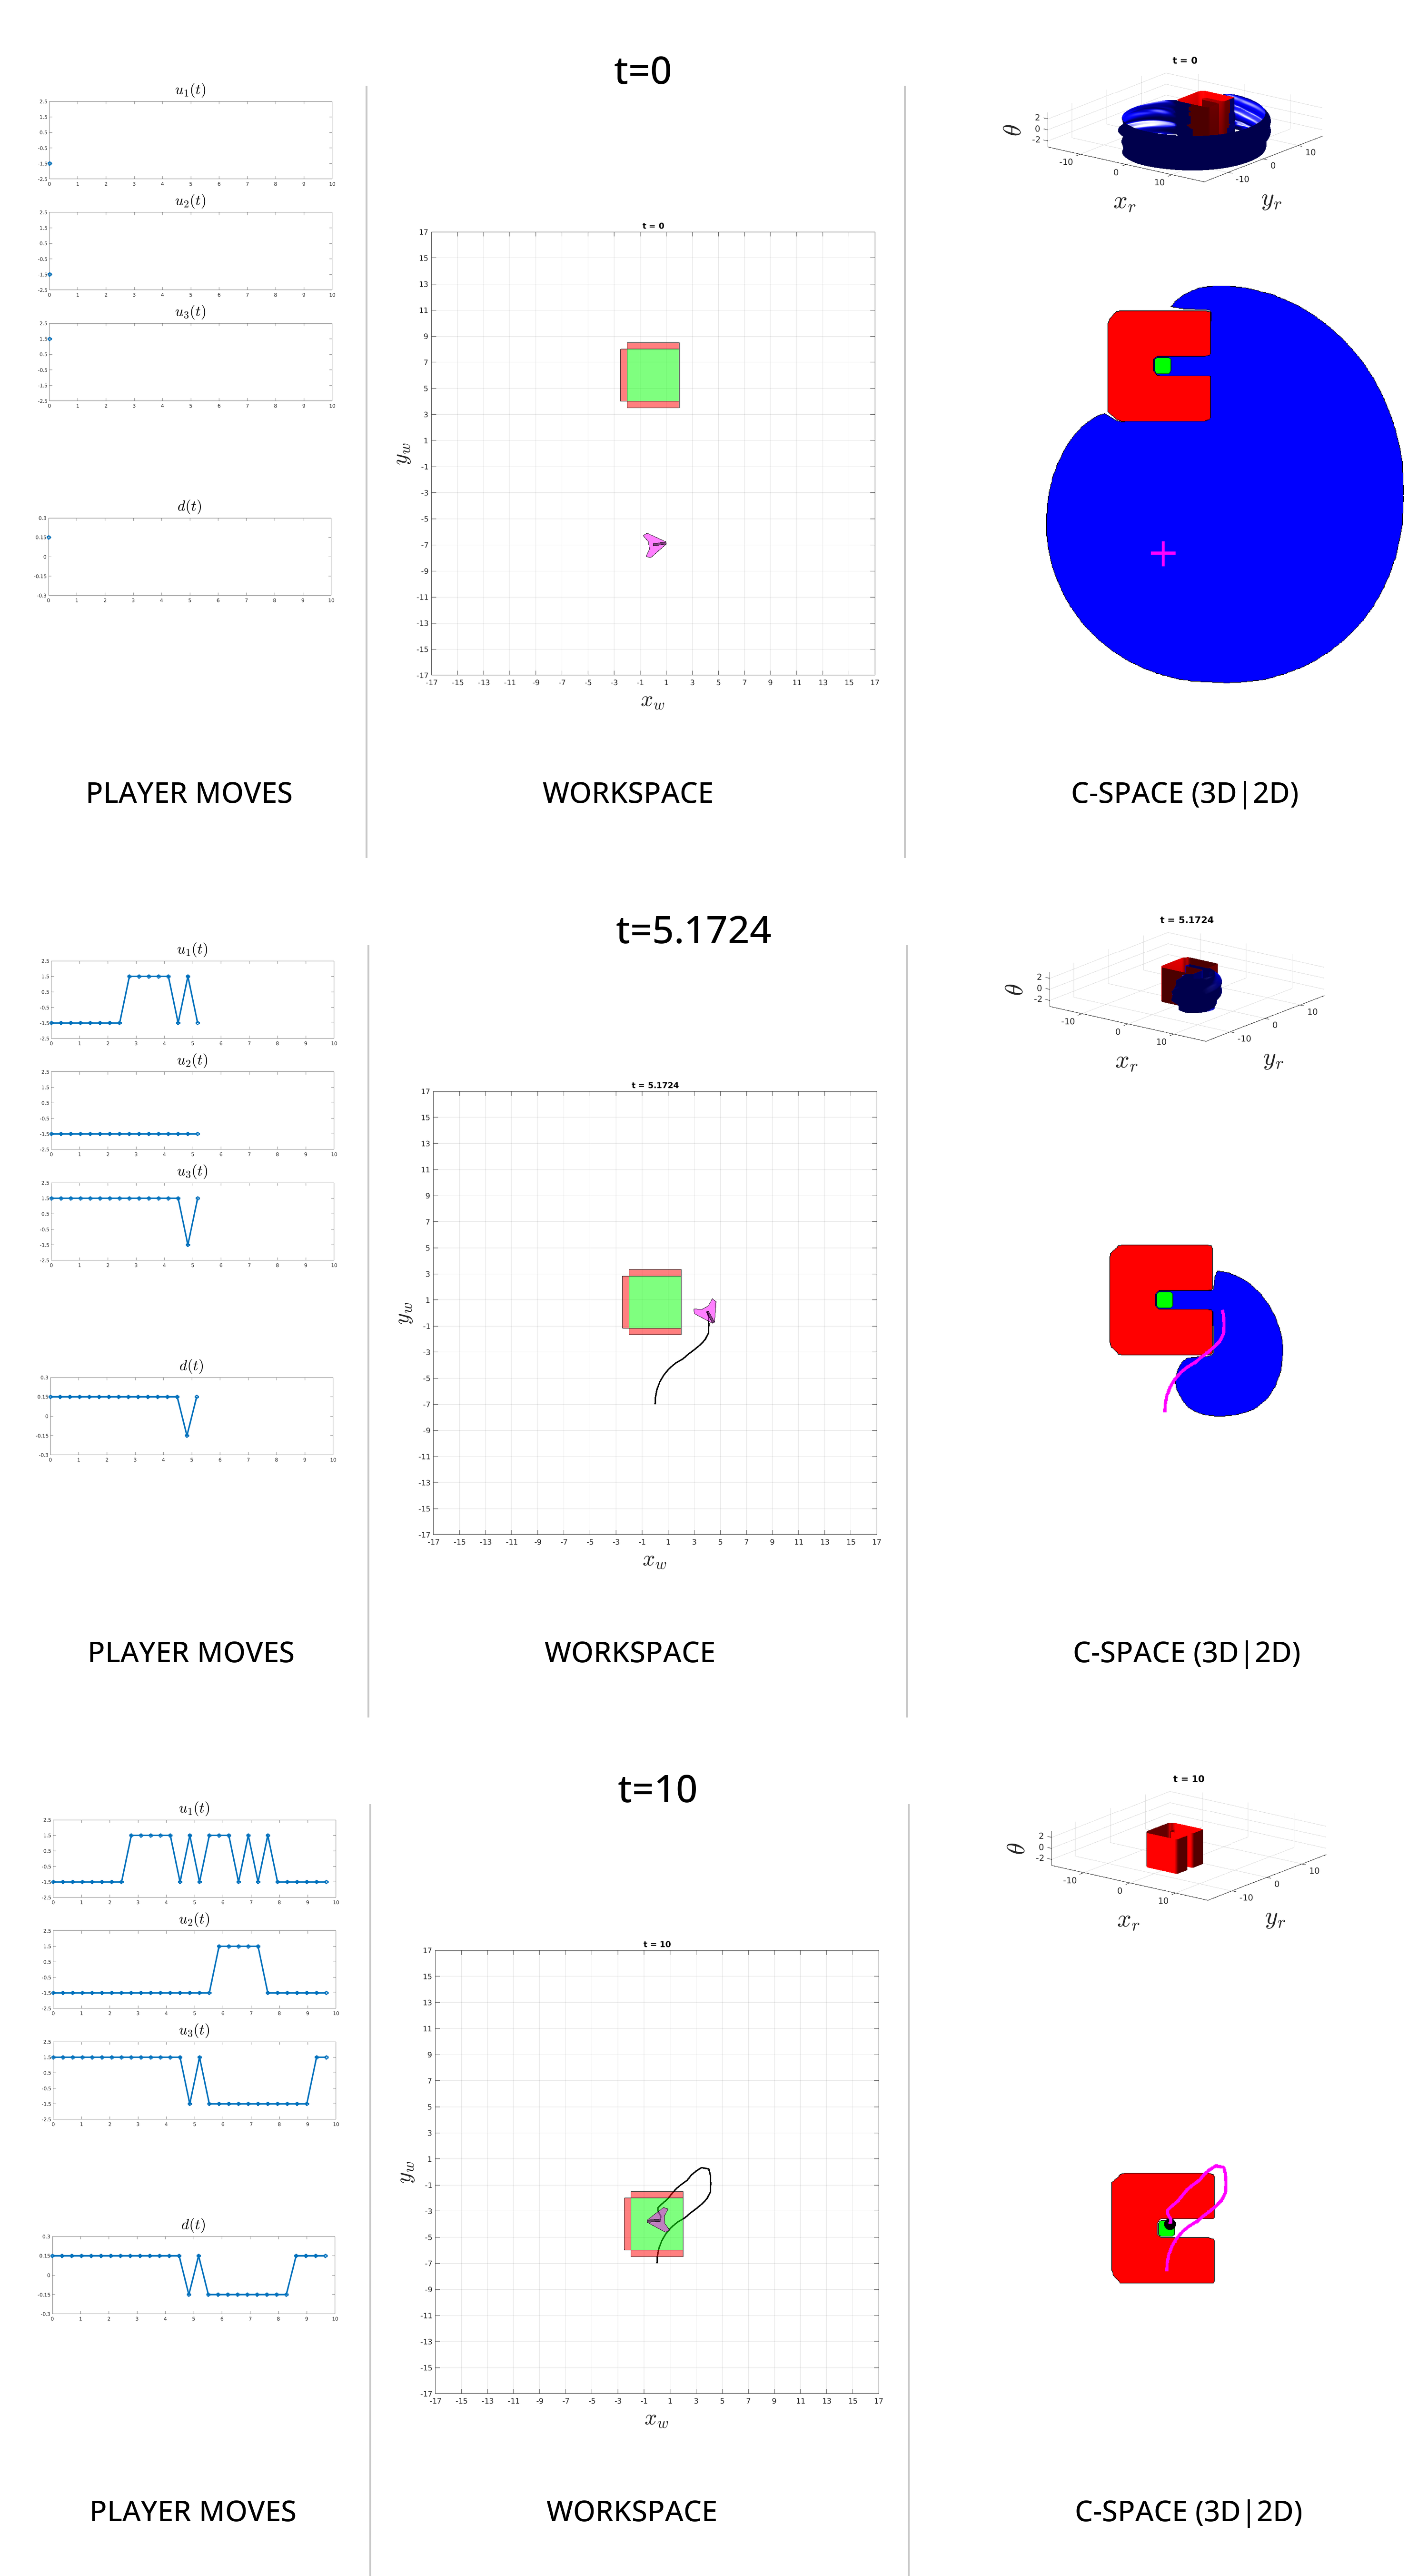
\includegraphics
        [width=0.7\textwidth]
        {figures/dynamic_faraway.png}
    \caption{Dynamic environment, optimal disturbance. $x_0 = [0, -7, -3]$, $\theta_d \in [-0.1, 0.1]$}
    \label{fig:dynamic_faraway}
\end{figure*}

\begin{figure*}[hp!]
    \centering
    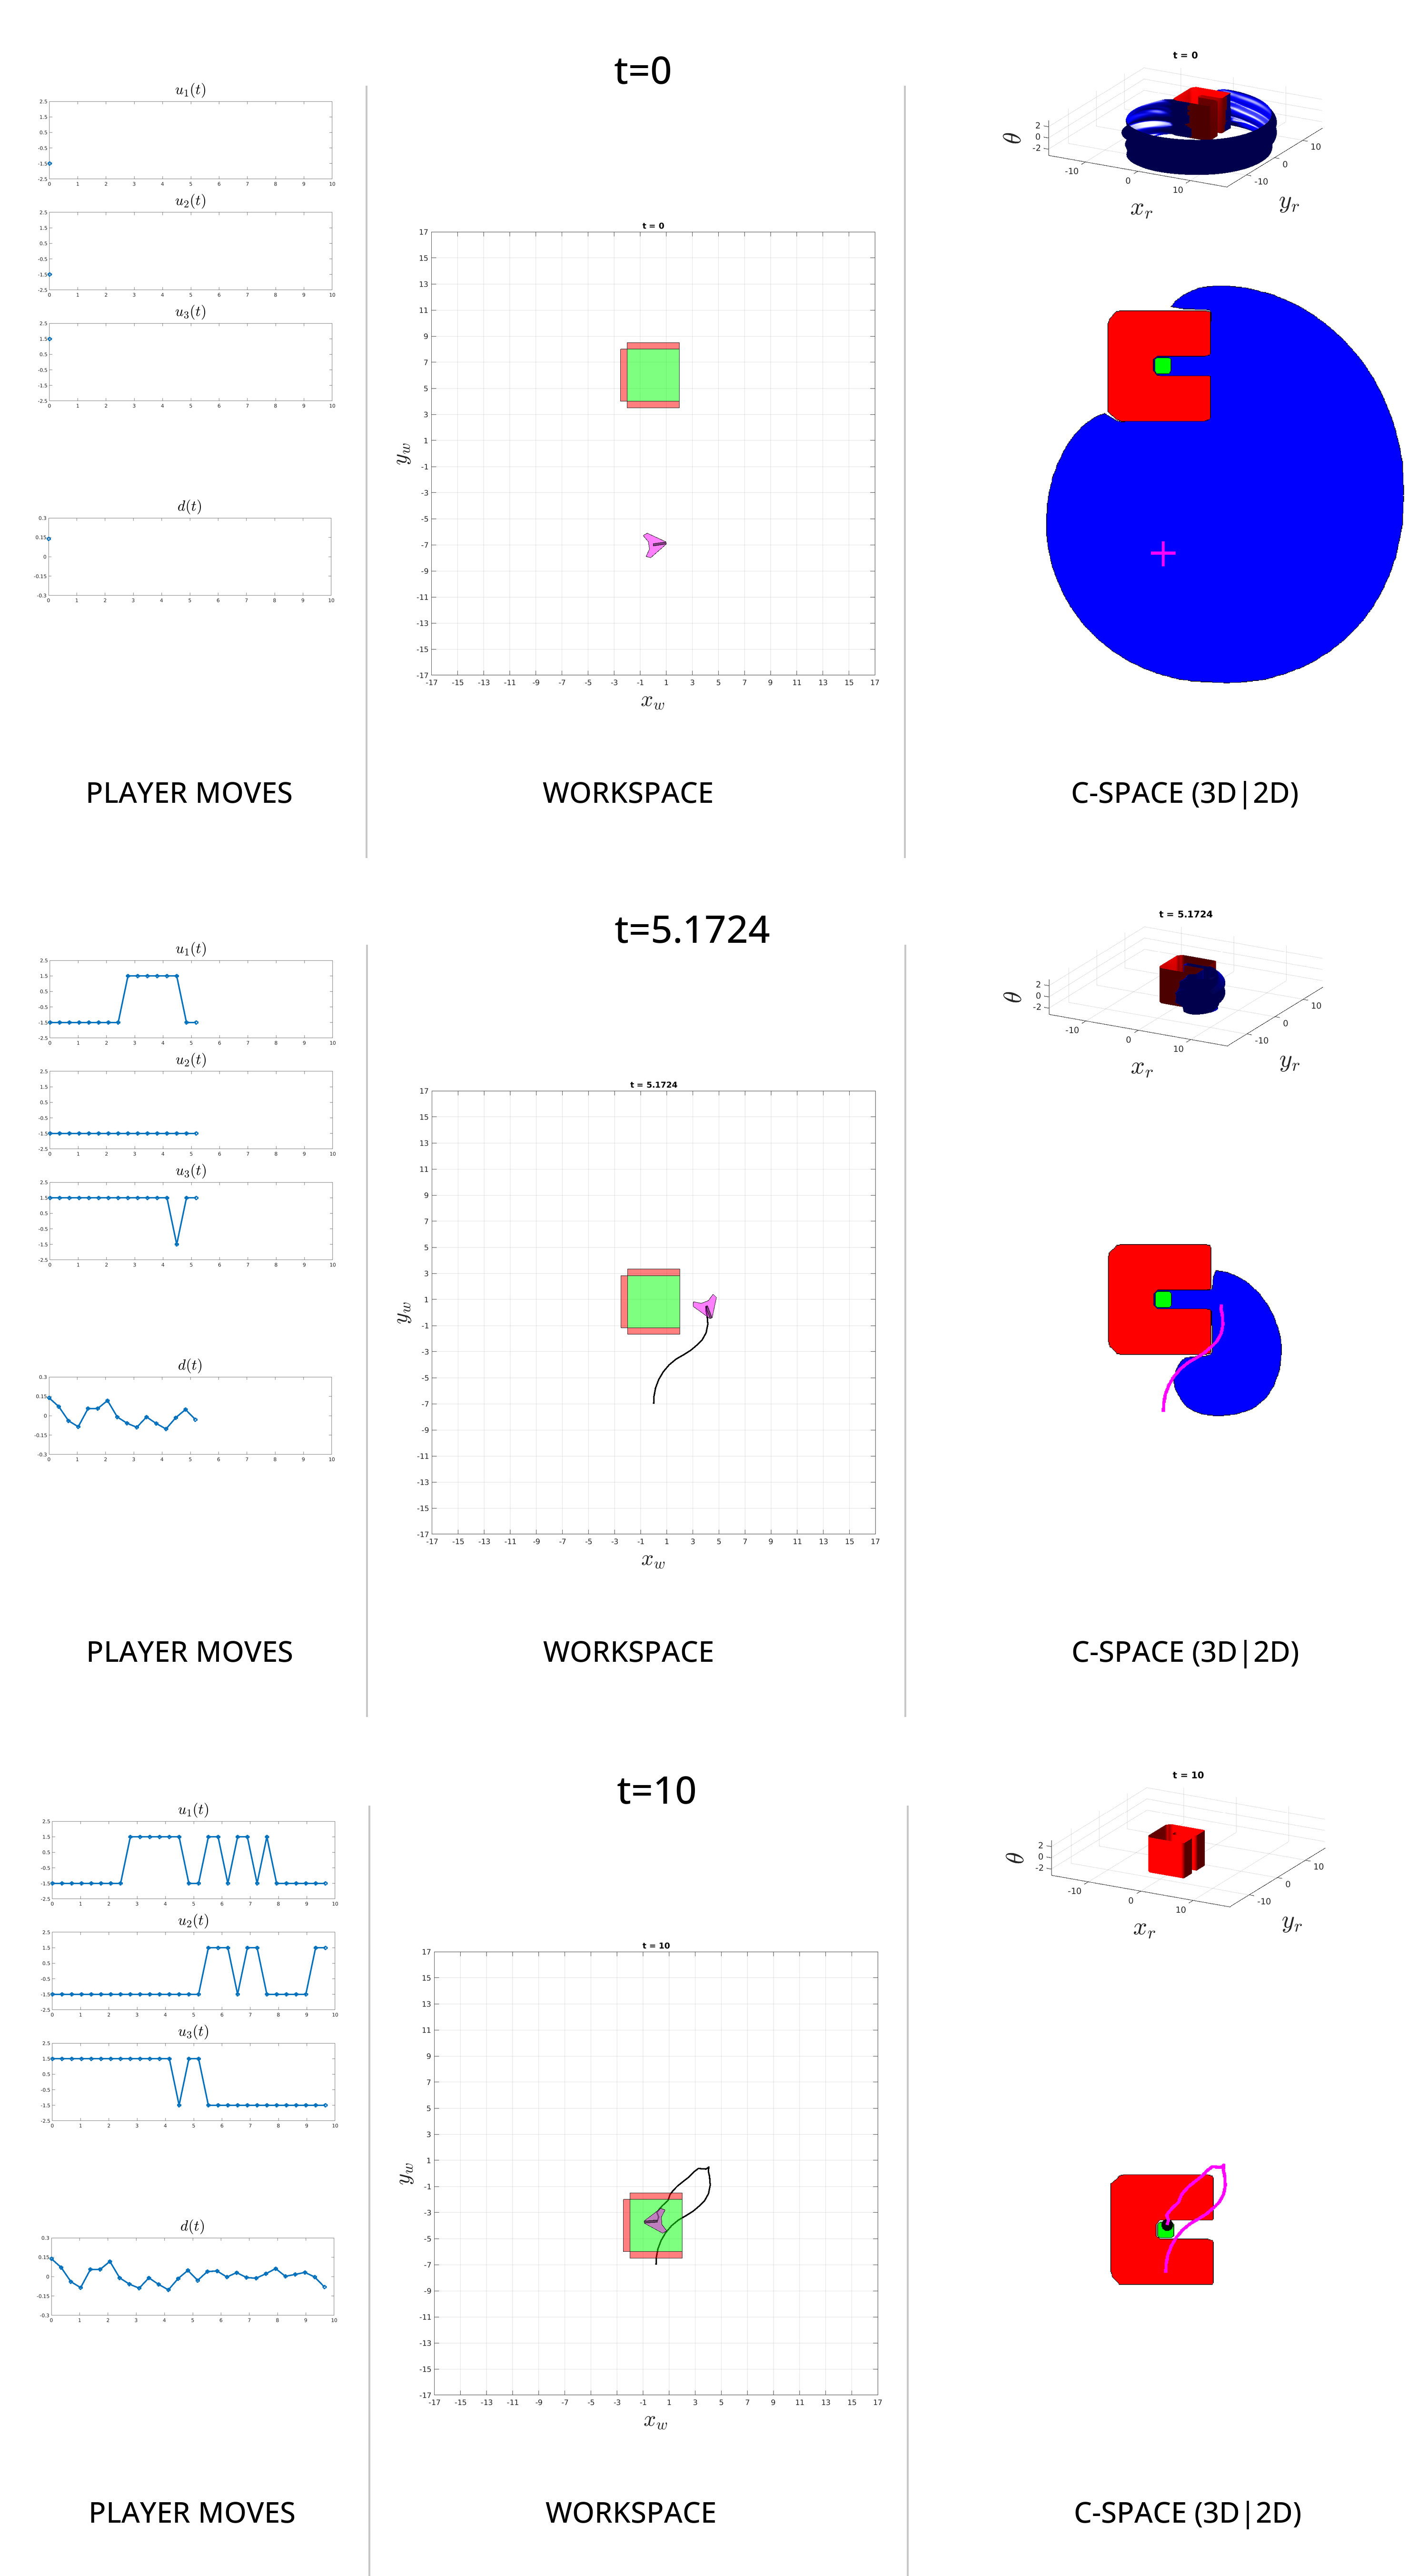
\includegraphics
        [width=0.7\textwidth]
        {figures/dynamic_faraway_ran.png}
    \caption{Dynamic environment, random disturbance. $x_0 = [0, -7, -3]$, $\theta_d \in [-0.1, 0.1]$}
    \label{fig:dynamic_faraway_ran}
\end{figure*}

\begin{figure*}[hp!]
    \centering
    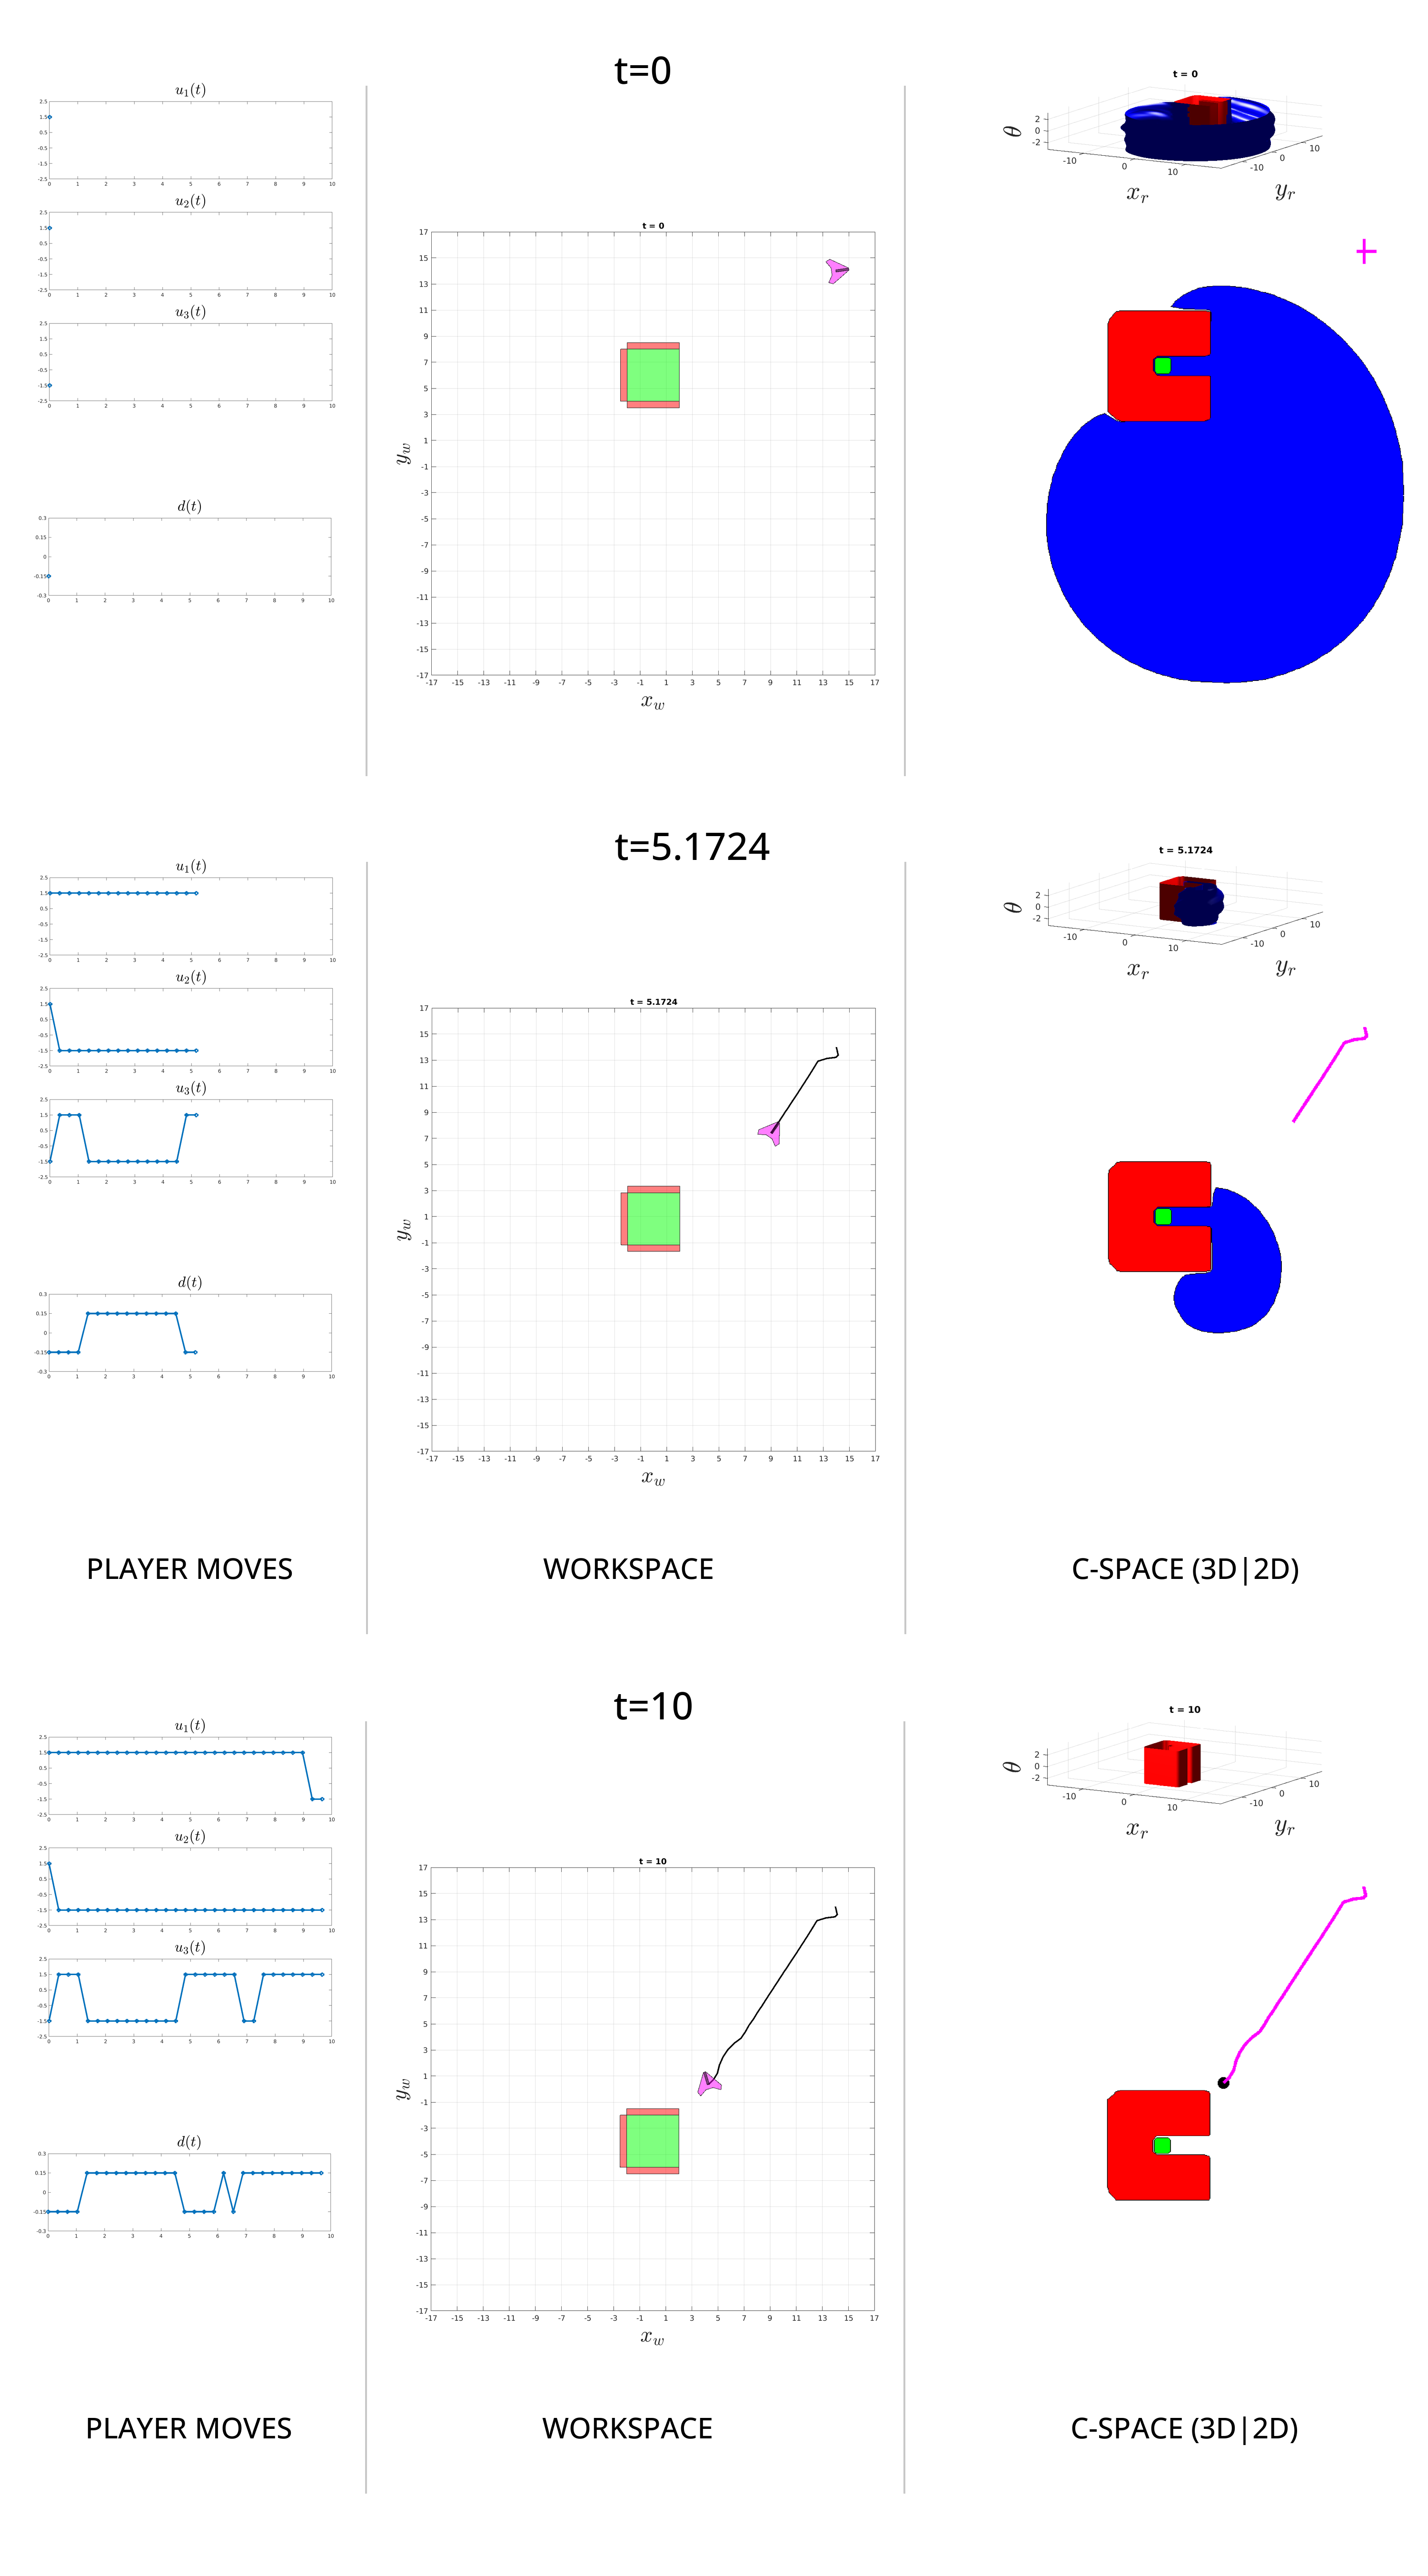
\includegraphics
        [width=0.7\textwidth]
        {figures/dynamic_outside_reach_avoid_set.png}
    \caption{Dynamic environment, optimal disturbance. $x_0 = [14, 14, -3]$, $\theta_d \in [-0.1, 0.1]$ (outside $RAS$)}
    \label{fig:dynamic_outside_reach_avoid_set}
\end{figure*}
